% pdflatex
\documentclass[hidelinks]{article}
\usepackage[a4paper, total={7in, 10in}]{geometry}
\usepackage[dvipsnames]{xcolor}
\usepackage{amsmath}
\usepackage{mathrsfs}

\usepackage{physics}
\let\qty\relax % 取消 physics 中定义的 \qty
\usepackage{siunitx}

\usepackage{tikz}
\usepackage{circuitikz}
\usepackage{tkz-euclide}
\usepackage[unicode]{hyperref}
%\usepackage[all]{hypcap}
\usepackage{fancyhdr}
\usepackage{float}
\pagestyle{fancy}

\DeclareMathOperator{\sgn}{sgn}

\fancyhead[L]{Yizhan Feng 2400017802}
\fancyhead[C]{}
\fancyhead[R]{\leftmark}

\usetikzlibrary{angles,calc, decorations.pathreplacing, arrows}

\title{\textbf{Electromagnetism Homework}}
\author{Yizhan Feng 2400017802}
\date{Spring, 2025}

\begin{document}
\hypersetup{bookmarksnumbered=true,}

\maketitle

\begin{Large}
\tableofcontents
\end{Large}%
\pagebreak



\section{Exercise W1}

\subsection{(1.41) \textit{Work for an octahedron}}
Three protons and three electrons are to be placed at the vertices of a regular octahedron of edge length $a$. We want to find the energy of the system, that is, the work required to assemble it starting with the particles very far apart. There are two essentially different arrangements. What is the energy of each?

\vspace{0.5cm}
\noindent
\textbf{Solution} \, Arrangement A: three protons are placed on one face of the octahedron to form a triangle:
$$U=\frac{e^2}{4\pi \varepsilon_0} \left(6\cdot\frac{1}{a} -6 \cdot \frac{1}{a} - 3\cdot \frac{1}{\sqrt{2}a} \right)= - \frac{3\sqrt{2}}{8\pi \varepsilon_0} \cdot \frac{e^2}{a}.$$
Arrangement B: two protons are placed on a pair of opposite vertices and one proton is at one of the rest four positions:
$$U=\frac{e^2}{4\pi \varepsilon_0} \left(4\cdot\frac{1}{a} + 2 \cdot \frac{1}{\sqrt{2}a} -8 \cdot \frac{1}{a} - \frac{1}{\sqrt{2}a} \right) = - \left(4- \frac{\sqrt{2}}{2}\right)\frac{1}{4\pi \varepsilon_0} \cdot \frac{e^2}{a}.$$


\subsection{(1.51) \textit{N charges on a circle}}
$N$ point charges, each with charge $Q/N$, are evenly distributed
around a circle of radius $R$. What is the electric field at the location of one of the charges, due to all the others? (You can leave
your answer in the form of a sum.) In the $N \to \infty$ limit, is the
field infinite or finite? In the $N \to \infty$ limit, is the force on one of the charges infinite or finite?

\vspace{0.5cm}
\noindent
\textbf{Solution} 

\begin{figure}[H]
    \centering
    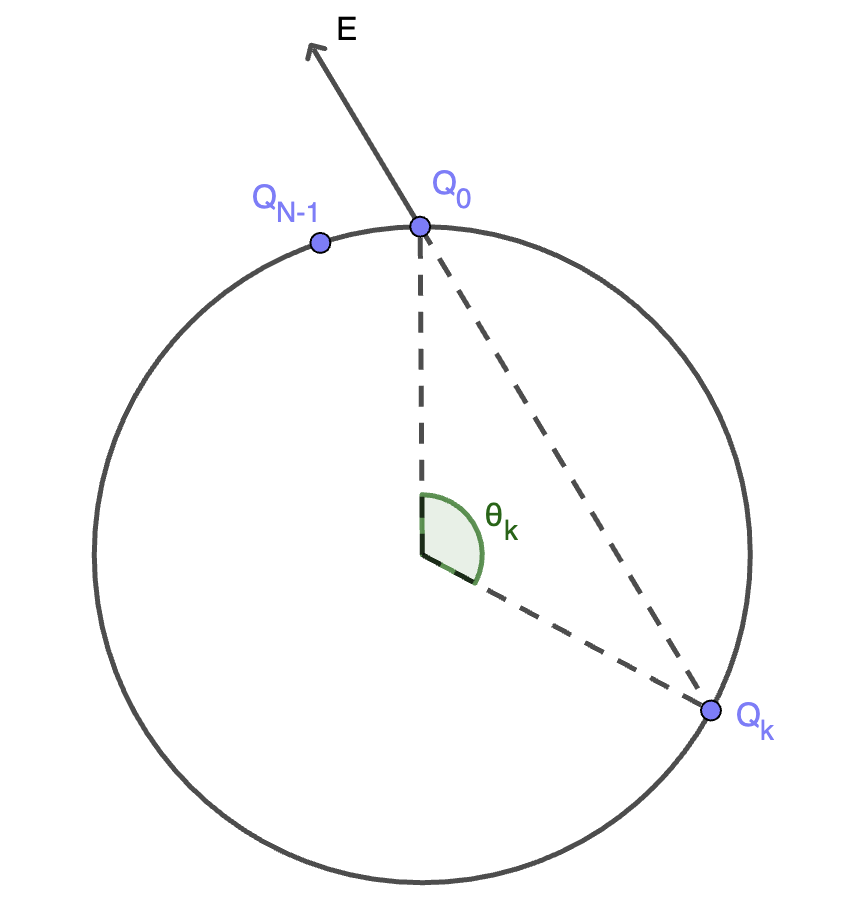
\includegraphics[width=0.3\linewidth]{Q1.51.png}
\end{figure}

Fix $Q_0$ as the origin of the reference frame. The circular symmetry requires the electric field at $Q_0$ to be only radial. Let $Q_k=2k\pi /N $ be the $k$-th charge on the circle, with a central angle $\theta_k$ with respect to $Q_0$. 
$$\abs{\va{r}_{k0}}=2R \sin \frac{\theta_k}{2}=2R \sin \frac{k\pi}{N}$$ 
$$E_k= \frac{Q/N}{4 \pi \varepsilon_0 \left(2R \sin \left(\frac{k\pi}{N} \right)    \right)^2} \cdot \sin \frac{\theta_k}{2}= \frac{Q/N}{16 \pi\varepsilon_0  R^2}\cdot \frac{1}{\sin \left(\frac{k\pi}{N} \right)}$$
Therefore, the total field at $Q_0$ is:
$$E=\sum_{k=1}^{N-1}E_k=\frac{Q}{16\pi\varepsilon_0 R^2} \sum_{k=1}^{N-1} \frac{1}{N\sin \left(\frac{k\pi}{N} \right)}=\frac{Q}{16\pi\varepsilon_0 R^2} \sum_{k=1}^{N} \frac{1}{N\sin \left(\frac{k\pi}{N} \right)}$$

In the limit $N\to\infty$, 
$$\lim_{N\to\infty} \sum_{k=1}^{N} \frac{1}{N \sin \left(\frac{k\pi}{N} \right)}=\frac{1}{\pi} \int_0^\pi \frac{\mathrm{d}x}{\sin x}=+\infty$$
so it's an infinite field.

The force on one charge is:
$$F=Eq=\frac{Q^2}{16\pi\varepsilon_0 R^2} \sum_{k=1}^{N} \frac{1}{N^2 \sin \left( \frac{k\pi}{N} \right)}$$
As $N\to \infty$,
$$\sum_{k=1}^{N} \frac{1}{N^2 \sin \left( \frac{k\pi}{N} \right)} \approx \sum_{k=1}^{N} \frac{1}{N^2 \cdot \left( \frac{k\pi}{N} \right)} = \frac{1}{N\pi} \sum_{k=1}^{N} \frac{1}{k} \sim \frac{1}{N\pi} \cdot \left( \ln N + \gamma + \order{\frac{1}{N}}\right)$$
which converges to $0$.

\subsection{(1.54) \textit{Semicircle and wires}}
(a) Two long, thin parallel rods, a distance $2b$ apart, are joined by a semicircular piece of radius $b$, as shown in Fig. 1.44. Charge of uniform linear density $\lambda$ is deposited along the whole filament. Show that the field $\vb{E}$ of this charge distribution vanishes at the point $C$. Do this by comparing the contribution of the element at $A$ to that of the element at $B$ which is defined by the same values of $\theta$ and $\mathrm{d}\theta$.\\
(b) Consider the analogous two-dimensional setup involving a
cylinder and a hemispherical end cap, with uniform surface
charge density $\sigma$. Using the result from part (a), do you think that the field at the analogous point $C$ is directed upward, downward, or is zero? (No calculations needed!)

\begin{figure}[H]
    \centering
    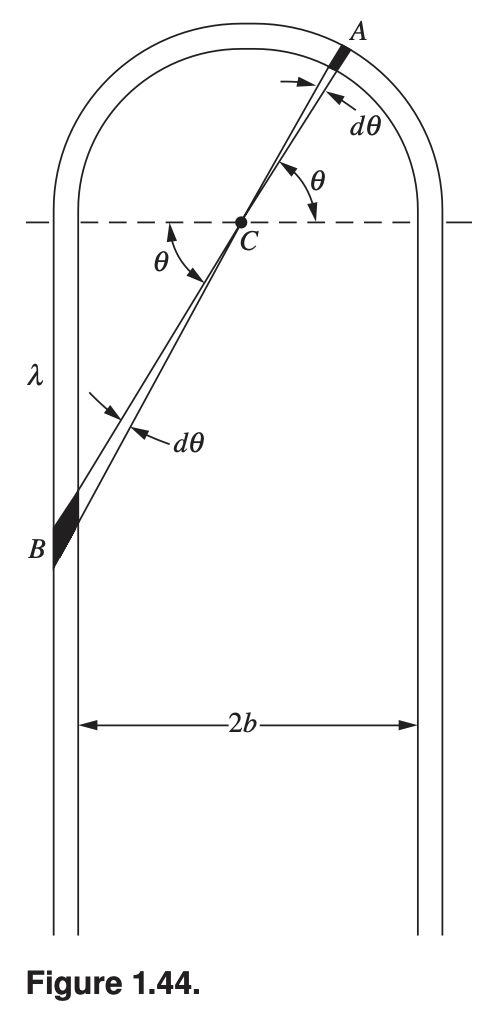
\includegraphics[width=0.3\linewidth]{F1.44.png}
\end{figure}

\vspace{0.5cm}
\noindent
\textbf{Solution} \, (a) $$E_A= \frac{1}{4\pi\varepsilon_0}\cdot \frac{Q}{r^2}=\frac{1}{4\pi\varepsilon_0}\cdot \frac{\lambda b \mathrm{d} \theta}{b^2} = \frac{1}{4\pi\varepsilon_0}\cdot \frac{\lambda \mathrm{d} \theta}{b}$$
$$E_B = \frac{1}{4\pi\varepsilon_0}\cdot \frac{Q'}{r'^2} = \frac{1}{4\pi\varepsilon_0}\cdot \frac{\lambda b \left[\tan \left(\theta + \mathrm{d}\theta \right) - \tan \theta \right]}{(b/\cos \theta)^2}$$
Note that $\mathrm{d} \theta \to 0$, 
$$\cos ^2 \theta \left[\tan \left(\theta + \mathrm{d}\theta \right) - \tan \theta \right] = \cos ^2 \theta \cdot \frac{\tan (\mathrm{d} \theta) \cdot (1+ \tan ^2 \theta)}{1-\tan \theta \cdot \tan (\mathrm{d} \theta)} \approx \tan (\mathrm{d} \theta) \sim \mathrm{d} \theta.$$
Therefore,
$$E_B = \frac{1}{4\pi\varepsilon_0}\cdot \frac{\lambda \mathrm{d} \theta}{b} = E_A,$$
and since they have opposite direction, the total field vanished at point $C$.\\[3mm]
(b) The field ar $C$ is directed upward. Consider a vertical slice of the cylinder and hemisphere which forms a planar charge distribution similar to (a). Unlike (a) where the rods have uniform width, the slice here becomes narrower towards the center of the hemisphere, eventually being zero at the center. This means that the downward field due to the upper semicircular part unable to fully cancel the upward field due to the lower linear part. So the total field is upward.


\subsection{(1.56) \textit{Flux through a cube}}
(a) A point charge $q$ is located at the center of a cube of edge $d$. What is the value of $\int \vb{E} \cdot \mathrm{d} \vb{a}$ over one face of the cube? \\
(b) The charge $q$ is moved to one corner of the cube. Now what
is the value of the flux of $\vb{E}$ through each of the faces of the cube? (To make things well defined, treat the charge like a tiny
sphere.)

\vspace{0.5cm}
\noindent
\textbf{Solution} \, (a) By Gauss's law, the total flux through $6$ faces of the cube is $q/\varepsilon_0$, so the flux through one face is $$\frac{1}{6} \int \vb{E} \cdot \mathrm{d} \vb{a} = \frac{q}{6\varepsilon_0}.$$\\[3mm]
(b) The spherical charge induces a field parallel to the $3$ faces that interact with it, so the flux through these $3$ faces is $0$. The total flux through the cube is equally shared by the rest $3$ faces, each being $$\frac{1}{3} \cdot \frac{\frac{1}{8}q}{\varepsilon_0}=\frac{q}{24\varepsilon_0}.$$



\subsection{(1.59) \textit{Zero field inside a cylindrical shell}}
Consider a distribution of charge in the form of a hollow circular cylinder, like a long charged pipe. In the spirit of Problem 1.17, show that the electric field inside the pipe is zero.

\vspace{0.5cm}
\noindent
\textbf{Solution} \, Consider a random point $P$ within the cylinder, and two patches on the cylinder shell defined by a pair of vertical angles at $P$. The two patches are similar by the ratio of the distances from $P$ to patches, namely $r_A$ and $r_B$. Therefore, $Q_A/Q_B=\sigma S_A/ \sigma S_B=r_A^2 / r_B^2 \implies E_A /E_B = (Q_A/r_A^2) / (Q_B/r_B^2) = 1$. Since $E_A$ and $E_B$ have opposite directions and the same magnitude, their fields cancel out, and so does every pair of similar patches. So, the electric field inside is $0$.

\subsection{(1.60) \textit{Field from a hollow cylinder}}
Consider the hollow cylinder from Exercise 1.59. Use Gauss’s law to show that the field inside the pipe is zero. Also show that the field outside is the same as if the charge were all on the axis. Is either statement true for a pipe of square cross-section on which the charge is distributed with uniform surface density?

\vspace{0.5cm}
\noindent
\textbf{Solution} \, Inside the cylinder, choose a cylindrical surface coaxial to the cylinder. The symmetry implies that $\vb{E}$ is radial and uniform on the surface. By Gauss's law, $$\int \vb{E} \cdot \mathrm{d} \vb{a} = E \cdot 2\pi rl = \frac{Q}{\varepsilon_0}.$$ Since no charge is enclosed in the cylinder, $Q=0 \implies E =0$.

Outside the cylinder, 
$$E \cdot 2\pi rl = \frac{Q}{ \varepsilon_0} = \frac{\sigma \cdot 2 \pi rl}{\varepsilon_0} \implies E= \frac{\sigma R}{\varepsilon_0 r},$$
which is equivalent to a line charge, where
$$E'=\frac {\lambda}{2\pi \varepsilon_0 r}, \quad \lambda= \sigma \cdot 2\pi R.$$ 

For a square cross-sectional pipe, the cylindrical symmetry is broken, so the fields inside, although yield $0$ when integrated over $\vb{a}$, are not radial and thus non-zero, and the fields outside do not resemble a line charge but depend on orientation relative to the pipe.

\pagebreak
\section{Exercise W2}
\subsection{(1.66) \textit{Force between two strips}}
(a) The two strips of charge shown in Fig. 1.47 have width $b$, infinite height, and negligible thickness (in the direction perpendicular to the page). Their charge densities per unit area are $\pm \sigma$. Find the magnitude of the electric field due to one of the strips, a distance $x$ away from it (in the plane of the page). \\
(b) Show that the force (per unit height) between the two strips equals $\sigma ^2 b(\ln 2) / \pi \varepsilon_0 $. Note that this result is finite, even though you will find that the field due to a strip diverges as you get close to it.

\begin{figure}[H]
    \centering
    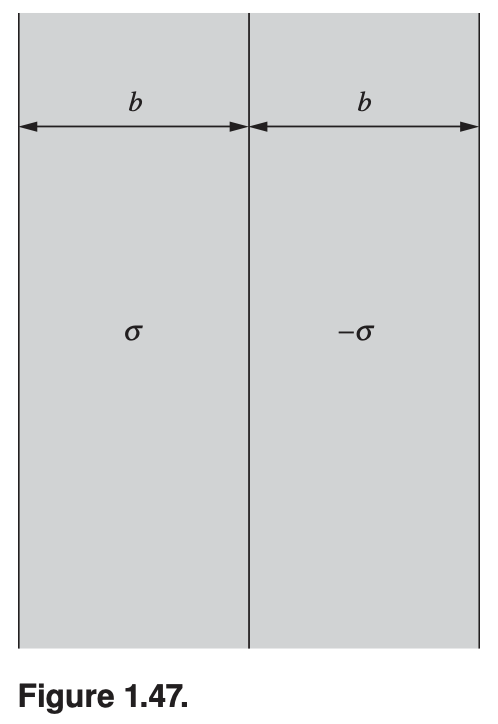
\includegraphics[width=0.3\linewidth]{F1.47.png}
\end{figure}

\vspace{0.5cm}
\noindent
\textbf{Solution} \, (a) Consider a narrow line on the strip, with width $\mathrm{d}r$ at a distance $r$ from the given point. By enclosing the line with a cylinder, the electric field at the point due to the narrow line can be deduced by Gauss's law:
$$E\cdot 2 \pi rL = \frac {\lambda L} {\varepsilon_0}  = \frac{\sigma L \mathrm{d}r}{{\varepsilon_0} }\implies E = \frac{\sigma \mathrm{d}r}{2\pi\varepsilon_0 r}.$$
Integrate it over the whole strip, the electric field at a distance $x$ from one strip is:
$$E=\int _x ^{x+b} \frac{\sigma \mathrm{d}r}{2\pi\varepsilon_0 r} = \frac{\sigma}{2 \pi \varepsilon_0} \ln \left( \frac{x+b}{x} \right).$$\\[3mm]
(b) A slice with width $\mathrm{d}x$, height $h$ and distance $x$ to the other strip contains charge of $\sigma h \mathrm{d}x$, so the force applied on it due to the other strip is: 
$$F_x = E(x) \cdot \sigma h \mathrm{d}x = \frac{\sigma^2h \mathrm{d}x}{2 \pi \varepsilon_0} \ln \left( \frac{x+b}{x} \right) .$$
Integrate it over the whole strip, the total force is:
\begin{align*}
    F & = \int _0 ^b F_x  = \frac{\sigma^2h }{2 \pi \varepsilon_0} \int_0^b  \ln \left( \frac{x+b}{x} \right) \mathrm{d}x \\& = \frac{\sigma^2h }{2 \pi \varepsilon_0} \left[ \int_0^b\ln(x+b) \mathrm{d}x-\int_0^b \ln x \mathrm{d}x \right] \\&=\frac{\sigma^2h }{2 \pi \varepsilon_0} \left[(2b\ln 2b -b\ln b -b) - (b\ln b - b)\right] \\&=\frac{\sigma^2h }{2 \pi \varepsilon_0} \cdot 2b\ln 2 \\&=\frac{\sigma^2 bh (\ln 2) }{ \pi \varepsilon_0}.
\end{align*}
Therefore, the force per unit height between the two strips is $\sigma ^2 b(\ln 2) / \pi \varepsilon_0 $.

\subsection{(1.69) \textit{Carved-out sphere}}
A sphere of radius $a$ is filled with positive charge with uniform density $\rho$. Then a smaller sphere of radius $a/2$ is carved out, as shown in Fig. 1.48, and left empty. What are the direction and magnitude of the electric field at $A$? At $B$?

\begin{figure}[H]
    \centering
    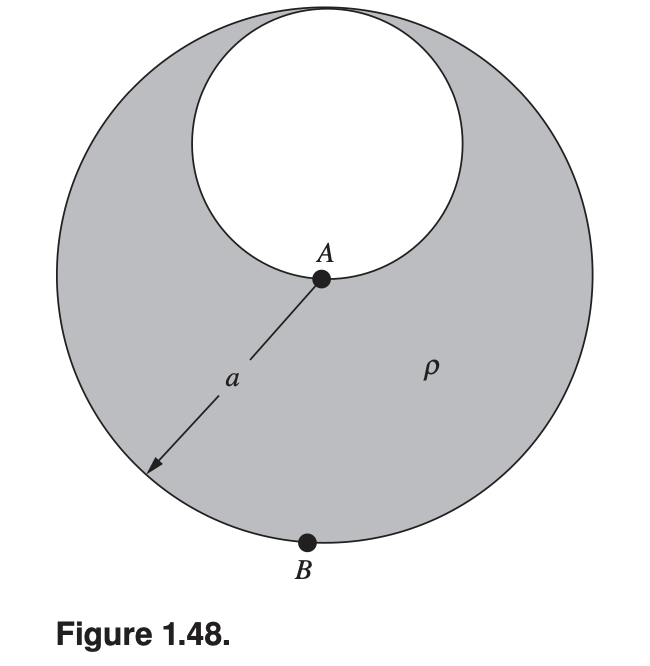
\includegraphics[width=0.3\linewidth]{F1.48.png}
\end{figure}

\vspace{0.5cm}
\noindent
\textbf{Solution} \,  The carved-out sphere is equivalent to placing a sphere of radius $a/2$ with uniform charge density $-\rho$ inside the bigger sphere.

At $A$, the field due to the bigger sphere is zero, and the field due to the smaller sphere is
$$E_{A,s} = \frac{-\rho (a/2)}{3\varepsilon_0}= -\frac{\rho a}{6\varepsilon_0}, $$
so the total electric field has magnitude
$$E_A = \left|E_{A,b} + E_{A,s} \right|= \frac{\rho a}{6\varepsilon_0},$$
and is directed upward.

At $B$, similarly, 
$$E_{B,b} = \frac{\rho a}{3\varepsilon_0},\quad E_{B,s}= \frac{-\rho (a/2)^3}{3\varepsilon_0 (3a/2)^2} = - \frac{\rho a}{54\varepsilon_0},$$
so the total electric field has magnitude
$$E_B = \left|E_{B,b}+E_{B,s} \right|= \frac{17\rho a}{54\varepsilon_0},$$
and is directed downward.

\subsection{(1.74) \textit{Zero field in a sphere}}
In Fig. 1.51 a sphere with radius $R$ is centered at the origin, an infinite cylinder with radius $R$ has its axis along the $z$ axis, and an infinite slab with thickness $2R$ lies between the planes $z =-R$ and $z=R$. The uniform volume densities of these objects are $\rho_1$, $\rho_2$, and $\rho_3$, respectively. The objects are superposed on top of each other; the densities add where the objects overlap. How should the three densities be related so that the electric field is zero everywhere throughout the volume of the sphere? Hint: Find a vector expression for the field inside each object, and then use superposition.

\begin{figure}[H]
    \centering
    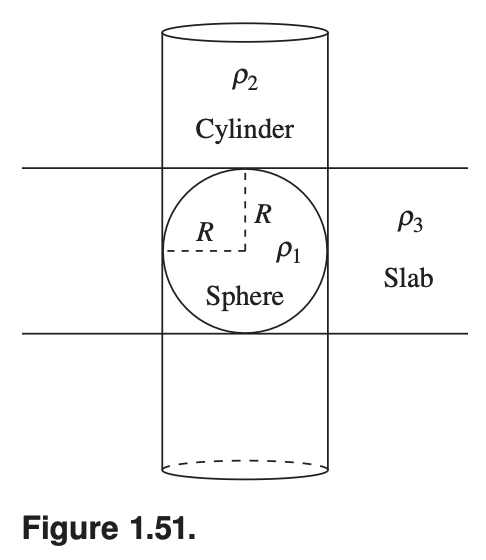
\includegraphics[width=0.26\linewidth]{F1.51.png}
\end{figure}

\vspace{0.5cm}
\noindent
\textbf{Solution} \, For any point $P(x,y,z)$ inside the sphere, the electric field due to the sphere can be deduced by Gauss's law:
$$E_{sphere} \cdot4\pi R^2 = \frac{\frac{4\pi R^3}{3} \rho _1} {\varepsilon_0} \implies E_{sphere} = \frac{R\rho_1}{3\varepsilon_0}\implies \vb{E}_{sphere} = E_{sphere} \cdot \vu{R}_{sphere}= \frac{R\rho_1}{3\varepsilon_0} \cdot (\vb{i},\vb{j},\vb{k}).$$
Similarly, the field due to the cylinder is:
$$E_{cylinder} \cdot 2\pi RL = \frac{\pi R^2L\rho_2}{\varepsilon_0} \implies E_{cylinder} = \frac{R\rho_2}{2\varepsilon_0} \implies \vb{E}_{cylidner} = E_{cylinder} \cdot \vu{R}_{cylinder} = \frac{R\rho_2}{2\varepsilon_0} \cdot (\vb{i},\vb{j},\vb{0}).$$
The field due to the slab is:
$$E_{slab} \cdot 2A = \frac{2RA\rho_3}{\varepsilon_0} \implies E_{slab} = \frac{R\rho_3}{\varepsilon_0} \implies \vb{E}_{slab} = E_{slab} \cdot \vu{R}_{slab} = \frac{R\rho_3}{\varepsilon_0} \cdot (\vb{0},\vb{0},\vb{k}).$$
These three fields add up to be zero, therefore:
$$
\left\{
\begin{aligned}
& \frac{1}{3} \cdot \rho_1 + \frac{1}{2} \cdot \rho_2 + 0\cdot \rho_3  = 0 \\
& \frac{1}{3} \cdot \rho_1+ \frac{1}{2} \cdot \rho_2 + 0\cdot \rho_3  = 0 \\
& \frac{1}{3} \cdot \rho_1+ 0 \cdot \rho_2 + 1\cdot \rho_3  = 0 \\
\end{aligned}
\right. \quad \implies  
\left\{
\begin{aligned}
& \rho_2 = - \frac{2}{3} \rho_1 \\
& \rho_3 = -\frac{1}{3} \rho_1
\end{aligned}
\right. .
$$

\subsection{(1.82) \textit{Energy of concentric shells}}
(a) Concentric spherical shells of radius $a$ and $b$, with $a < b$, carry charge $Q$ and $-Q$, respectively, each charge uniformly distributed. Find the energy stored in the electric field of this system. \\
(b) Calculate the stored energy in a second way: start with two neutral shells, and then gradually transfer positive charge from the outer shell to the inner shell in a spherically symmetric manner. At an intermediate stage when there is charge $q$ on the inner shell, find the work required to transfer an additional charge $\mathrm{d}q$. And then integrate over $q$.

\vspace{0.5cm}
\noindent
\textbf{Solution} \, (a) By Gauss's law, the electric field should be zero in the region $r>b$ and $r<a$, and within the region $a<r<b$, the field is $E=Q/4\pi r^2 \varepsilon_0$. Therefore the energy is:
$$U = \frac{\varepsilon_0}{2} \int E^2\mathrm{d}V= \frac{\varepsilon_0}{2} \int_a^b \left( \frac{Q}{4\pi r^2 \varepsilon_0} \right)^2 \cdot 4\pi r^2 \mathrm{d}r = \frac{Q^2}{8\pi \varepsilon_0} \int_a^b \frac{\mathrm{d}r}{r^2} = \frac{Q^2}{8\pi \varepsilon_0} \left(\frac{1}{a} - \frac{1}{b}\right).$$\\[3mm]
(b) At the moment when charge $q$ is transferred to the inner shell, the electric field between the two shells is $E = q/4\pi r^2 \varepsilon_0$. To transfer another $\mathrm{d}q$, the force to be applied is $F = -E \cdot \mathrm{d}q = -q \cdot \mathrm{d}q/4\pi r^2 \varepsilon_0$, so the work required can be deduced by integrating $F$ over $r$ from $b$ to $a$:
$$\mathrm{d}W = \int _b^a -\frac{q \cdot \mathrm{d}q}{4\pi r^2 \varepsilon_0} \mathrm{d}r = \frac{q\cdot \mathrm{d}q}{4\pi \varepsilon_0} \left(\frac{1}{a}-\frac{1}{b} \right).$$
Then integrate $\mathrm{d}W$ over $q$, the total work is:
$$W = \int_0^Q \mathrm{d}W = \int_0^Q \frac{q\cdot \mathrm{d}q}{4\pi \varepsilon_0} \left(\frac{1}{a}-\frac{1}{b} \right) = \frac{Q^2}{8\pi \varepsilon_0} \left(\frac{1}{a} - \frac{1}{b}\right),$$
which is consistent with (a).

\pagebreak
\section{Exercise W3}
\subsection{(2.35) \textit{Center vs. corner of a square}} 
A square sheet has uniform surface charge density $\sigma$. Letting the electric potential $\phi$ be zero at infinite distance from the square, denote by $\phi_0$ the potential at the center of the square and by $\phi_1$ the potential at a corner. Determine the ratio $\phi_0/\phi_1$. The answer can be found with very little calculation by combining a dimensional argument with superposition. (Think about the potential at the center of a square with the same charge density and with twice the edge length.)

\vspace{0.5cm}
\noindent
\textbf{Solution} \, Generally, the electric potential $\phi$ at a point is proportional to the total charge $Q$ and inversely proportional to a characteristic length $r$. Here the characteristic length of the square sheet should be its side length, $a$, and its total charge of the square sheet is $\sigma a^2$. Therefore,
$$\phi \propto \frac{Q}{r} = \frac{\sigma a^2}{a}=\sigma a .$$
Consider a larger square with edge length $2a$. The center of this larger square is equivalent to the corner of each of the four smaller squares that make up the larger square. So the potential at the center of the larger square is the sum of the potentials from each of the four smaller squares:
$$\phi_c = 4\phi_1.$$
On the other hand, the potential at the center of the large square should also be proportional to $\sigma \cdot 2a$, which is twice the potential at the center of the smaller square with side length $a$. Therefore,
$$\phi_c = 2\phi_0.$$
This indicates that $\phi_0/\phi_1=2$.

\subsection{(2.53) \textit{Field from two shells}} 
One of two nonconducting spherical shells of radius $a$ carries a charge $Q$ uniformly distributed over its surface, the other carries a charge $-Q$, also uniformly distributed. The spheres are brought together until they touch. What does the electric field look like, both outside and inside the shells? How much work is needed to move them far apart?

\vspace{0.5cm}
\noindent
\textbf{Solution} \, The electric field outside the two shells is the same as a field due to two point charges $Q$ and $-Q$ located at two centers of the shell. The field inside each shell is the same as a field due a point charge located at the center of the other shell.

Since the charged shell is equivalent to a point charge located at the center in regard to its external field, the work required to move two shells apart is the same as moving two point charges from $2a$ to infinitely apart. Therefore,
$$W= \frac{1}{4\pi\varepsilon_0} \frac{Q^2}{2a}.$$

\subsection{(2.62) \textit{Square quadrupole}}
Consider a square quadrupole consisting of two adjacent dipoles oppositely oriented and placed side by side to form a square, as shown in Fig. 2.16. If the side length is $l$, find the electric field at a large distance $r$ along the diagonal containing the two positive charges. Be careful to take into account all quantities that are second order in $l/r$.
\begin{figure}[H]
    \centering
    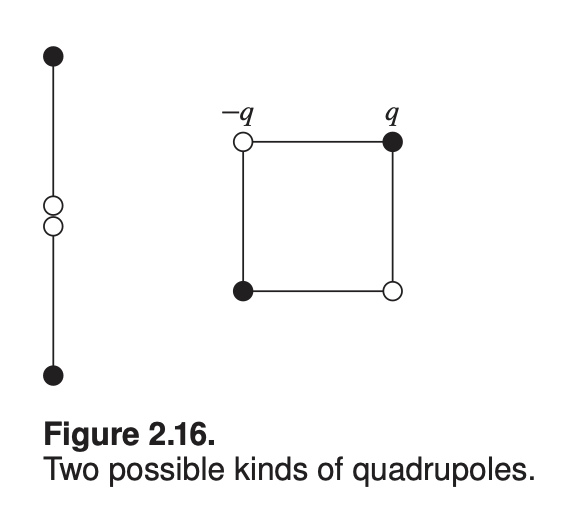
\includegraphics[width=0.3\linewidth]{F2.16.png}
\end{figure}

\vspace{0.5cm}
\noindent
\textbf{Solution}
\begin{figure}[H]
    \centering
    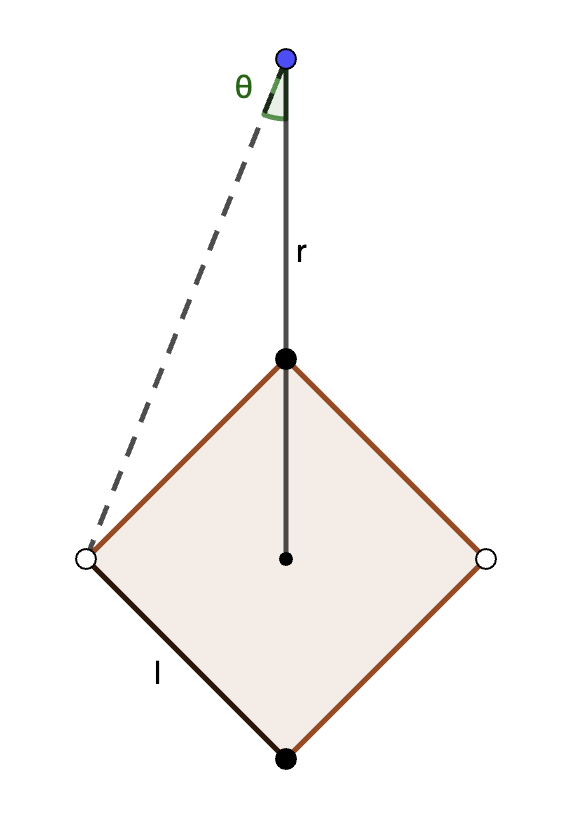
\includegraphics[width=0.3\linewidth]{Q2.62.png}
\end{figure}
By symmetry, the electric field at this point is radial.
\begin{align*}
    E &= \frac{q}{4\pi\varepsilon_0} \left[ \frac{1}{\left(r-l/\sqrt{2}\right)^2} + \frac{1}{\left(r+l/\sqrt{2}\right)^2} - 2 \frac{\cos \theta}{r^2+l^2/2} \right] \\
    &= \frac{q}{4\pi\varepsilon_0 r^2} \left[ \frac{1}{\left(1-l/\sqrt{2}r\right)^2} + \frac{1}{\left(1+l/\sqrt{2}r\right)^2} - \frac{2}{\left(1+\left(l/\sqrt{2}r\right)^2\right)^{3/2}} \right] \\ 
    &\approx \frac{q}{4\pi\varepsilon_0 r^2} \left[\left(1+2 \left( l/\sqrt{2}r\right) +3\left(l/\sqrt{2}r\right)^2 \right) + \left( 1-2\left(l/\sqrt{2}r\right) +3\left(l/\sqrt{2}r\right)^2 \right) - \left( 2-3\left(l/\sqrt{2}r\right)^2\right) \right] \\
    & = \frac{9ql^2}{8\pi\varepsilon_0r^4}.
\end{align*}
The field is directed away from the quadrupole.

\subsection{(2.69) \textit{$\boldsymbol{E}$ and $\boldsymbol{\phi}$ for a slab}}
A rectangular slab with uniform volume charge density $\rho$ has thickness $2l$ in the $x$ direction and infinite extent in the $y$ and $z$ directions. Let the $x$ coordinate be measured relative to the center plane of the slab. For values of $x$ both inside and outside the slab: \\[3mm]
(a) find the electric field $E(x)$ (you can do this by considering the amount of charge on either side of $x$, or by using Gauss’s law); \\
(b) find the potential $\phi(x)$, with $\phi$ taken to be zero at $x = 0$; \\
(c) verify that $\rho(x)= \varepsilon_0 \div{\vb{E}(x)}$ and $\rho(x)=-\varepsilon_0 \laplacian{\phi(x)}$.

\vspace{0.5cm}
\noindent
\textbf{Solution} \, (a) At position $x$ inside the slab, consider two Gaussian surfaces enclosing slab parts left and right to $x$. The electric field at $x$ is the sum of two slab parts:
$$E(x) = \frac{(l+x)\rho}{2\varepsilon_0} - \frac{(l-x)\rho}{2\varepsilon_0} = \frac{\rho x}{\varepsilon_0},$$
and is directed away from the center plane. Outside the slab, consider a single Gaussian surface enclosing the whole slab. The electric field at $x$ is:
$$E(x) = \frac{2\rho l}{2\varepsilon_0} \cdot \sgn(x) = \frac{\rho l  }{\varepsilon_0} \cdot \sgn (x).$$
Therefore,
$$E(x) =  \left\{
\begin{aligned}
& \frac{\rho x}{\varepsilon_0} & \quad \abs{x}\leq l \\ 
& \frac{\rho l}{\varepsilon_0}\cdot\sgn (x) & \quad \abs{x}>l
\end{aligned}
\right. .
$$\\
(b) Inside the slab, the potential relative to the center is:
$$\phi(x) = -\int_0^{\abs{x}} \frac{\rho x}{\varepsilon_0} \, \mathrm{d}x = -\frac{\rho x^2}{2\varepsilon_0}. $$
Outside the slab, the potential relative to the center is:
$$\phi(x) = -\int_0^{l} \frac{\rho x}{\varepsilon_0} \, \mathrm{d}x - \int _l ^ {\abs{x}} \frac{\rho l}{\varepsilon_0} \, \mathrm{d}x = \frac{\rho l^2}{2\varepsilon_0} - \frac{\rho l \abs{x}}{\varepsilon_0}.$$
Therefore,
$$\phi(x) =  \left\{
\begin{aligned}
& -\frac{\rho x^2}{2\varepsilon_0} & \quad \abs{x}\leq l \\ 
& \frac{\rho l^2}{2\varepsilon_0}-\frac{\rho l \abs{x}}{\varepsilon0} & \quad \abs{x}>l
\end{aligned}
\right. .
$$\\
(c) Both are indeed correct:
$$\varepsilon_0 \div{\vb{E}(x)} = \varepsilon_0 \frac{\partial E(x)}{\partial x} = \left\{
\begin{aligned}
    &\rho &\quad \abs{x}\leq l \\
    & 0 & \quad \abs{x} >l
\end{aligned}
\right. \, = \rho(x).
$$
$$\varepsilon_0 \laplacian{\phi(x)} = \varepsilon_0 \frac{\partial^2 \phi(x)}{\partial x^2} = \left\{
\begin{aligned}
    &\rho &\quad \abs{x}\leq l \\
    & 0 & \quad \abs{x} >l
\end{aligned}
\, = \rho(x)
\right..
$$

\pagebreak

\section{Exercise W4}
\subsection{(2.67) \textit{Product of $\boldsymbol{\rho}$ and $\boldsymbol{\phi}$}}
Consider a charge distribution $\rho_1(\vb{r})$ and the potential $\phi_1(\vb{r})$ due to it. Consider another charge distribution $\rho_2(\vb{r})$ and the potential $\phi_2(\vb{r})$ due to it. Both distributions have finite extent, but are otherwise arbitrary and need not have anything to do with each other. Show that $\int \rho_1 \phi_2 \, \mathrm{d}v = \int \rho_2 \phi_1 \, \mathrm{d}v$, where the integrals are taken over all space. Solve this in two different ways as follows.\\[3mm]
(a) Consider the two collections of charges to be rigid objects that
can be moved around. Start with them initially located very far
apart, and then bring them together. How much work does this
require? Imagine moving collection 1 toward collection 2, and
then the other way around. \\
(b) Consider the integral $\int \vb{E}_1 \vb{E}_2 \, \mathrm{d}v$ over all space, where $\vb{E1}$ and $\vb{E}_2$ are the electric fields due to the two distributions. By using the vector identity $\div (\vb{E}_1 \phi_2) = (\div \vb{E}_1) \phi_2 + \vb{E}_1 \cdot \grad \phi_2$ (and similarly with the 1s and 2s switched), rewrite the integral $\int \vb{E}_1 \vb{E}_2 \, \mathrm{d}v$ in two different ways.

\vspace{0.5cm}
\noindent
\textbf{Solution} \, (a) By bringing charges of collection 1 from infinitely apart to close up together, an element of charge in collection 1, $\mathrm{d}q = \rho_1 \, \mathrm{d}v$, gains an energy of $\phi_2 \, \mathrm{d}q = \rho_2 \phi_2 \, \mathrm{d}v$. Therefore, the integral $\int \rho_1 \phi_2 \, \mathrm{d}v$ represents the total work done. The same reasoning can be applied to the process of bring charges of collection 2 from infinitely apart to close up together, in which the work done is $\int \rho_2 \phi_1 \, \mathrm{d}v$. Since the amount of work doesn't depend on the process, the two integrals should be equal. \\[3mm]
(b) Since $\div \vb{E}_1 = \rho_1 / \varepsilon_0$ and $\vb{E_2} = -\grad \phi_2$, the vector identity can be rewritten as
$$\div{(\vb{E}_1 \phi_2)} = \frac{\rho_1 \phi_2}{\varepsilon_0} - \vb{E}_1  \vb{E}_2.$$
By Gauss's theorem, the integral
$$\int \div (\vb{E}_1 \phi_2) \, \mathrm{d}v = \int \vb{E}_1 \phi_2 \, \mathrm{d}\vb{a}$$
should vanish at infinity, because the charge distributions $\rho_1$ and $\rho_2$ are of finite extent, and thus their potentials $\phi_1$ and $\phi_2$ fall off to zero at sufficiently large distance. Therefore, integrating the vector identity over all space yield
$$ \frac{1}{\varepsilon_0} \int \rho_1 \phi_2 \, \mathrm{d}v = \int \vb{E}_1 \vb{E}_2 \, \mathrm{d}v.$$
Proceed similarly with 1s and 2s switched. It should yield
$$ \frac{1}{\varepsilon_0} \int \rho_2 \phi_1 \, \mathrm{d}v = \int \vb{E}_1 \vb{E}_2 \, \mathrm{d}v.$$
Therefore, $\int \rho_1 \phi_2 \, \mathrm{d}v = \int \rho_2 \phi_1 \, \mathrm{d}v$.

\subsection{(3.47) \textit{Bump on a plane}}
An infinite conducting plane has a hemispherical bump on it with radius $R$. A point charge $Q$ is located a distance $R$ above the top of the hemisphere, as shown in Fig. 3.33. With the help of Problem 3.13, find the image charges needed to make the electric field perpendicular to the plane and the hemisphere at all points.
\begin{figure}[H]
    \centering
    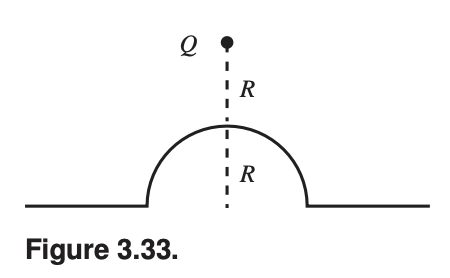
\includegraphics[width=0.3\linewidth]{F3.33.png}
\end{figure}

\vspace{0.5cm}
\noindent
\textbf{Solution} \, First, to ensure that the plane remains an equipotential surface, a charge $-Q$ located at a distance $R$ below the plane (i.e., at $(0,0,-2R)$). This also makes the potential over the whole conducting surface uniformly zero.

The conducting hemisphere must also be an equipotential, meaning that there will be an extra pair of image charges placed at $z$ axis that cancel the field at its surface. Consider an image charge $-q$ at $(0,0,z)$. The potential at $(0,0,R)$ is
$$\phi = \frac{1}{4\pi\varepsilon_0} \left( \frac{Q}{R} - \frac{q}{R-d} \right) = 0.$$
The potential at $(R,0,0)$ is also
$$\phi = \frac{1}{4\pi \varepsilon_0 } \left( \frac{Q}{
\sqrt{5}R} -\frac{q}{\sqrt{d^2+R^2}}\right)=0.$$
The two equations solve to $d=R/2$ and $q=Q/2$. Symmetrically, an additional image charge $q=Q/2$ should be place at $(0,0,-d) = (0,0,-R/2)$ to maintain the plane equipotential.

To sum up, three image charges are needed: $-Q/2$ at $(0,0,R/2)$, $Q/2$ at $(0,0,-R/2)$ and $-Q$ at $(0,0,-2R)$.

\subsection{(3.55) \textit{Two pairs of plates}}
Four conducting plates lie parallel to each other, as shown in Fig. 3.38. The spacings between them are arbitrary (but small compared with the lateral dimensions). The top two plates are connected by a wire so that they are at the same potential, and likewise for the bottom two. A total charge $Q_1$ resides on the top two plates, and a total charge $Q_2$ on the bottom two. What is the charge on each of the four plates?
\begin{figure}[H]
    \centering
    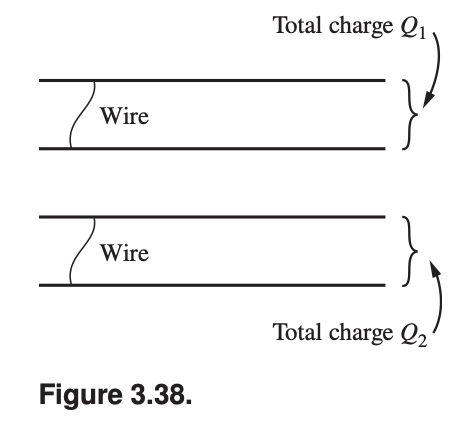
\includegraphics[width=0.3\linewidth]{F3.38.png}
\end{figure}

\vspace{0.5cm}
\noindent
\textbf{Solution} \, Let four plates be denoted as plate A, B, C and D from up to down. First enclose plate B and C with a Gaussian surface. Since $E=0$ between the two connected pairs of plate, the total flux of the Gaussian surface is zero. This indicates that $q_B+q_C = 0$. On the other hand, the two outer plate, A and D, must have same charge to maintain a net zero field in both $E=0$ region. Therefore,
$$
\begin{aligned}
    q_A &= q_D \\
    q_B+q_C &= 0 \\ 
    q_A+q_B &= Q_1 \\ 
    q_C+q_D &= Q_2
\end{aligned}
\implies
\left\{
\begin{aligned}
    q_A = \frac{Q_1+Q_2}{2} \\ 
    q_B = \frac{Q_1-Q_2}{2} \\
    q_C = \frac{Q_2-Q_1}{2} \\
    q_D = \frac{Q_1+Q_2}{2} 
\end{aligned}
\right..
$$

\subsection{(3.59) \textit{Coaxial capacitor}}
A capacitor consists of two coaxial cylinders of length $L$, with outer and inner radii $a$ and $b$. Assume $L \gg a-b$, so that end corrections may be neglected. Show that the capacitance is $C=2\pi \varepsilon_0 L/ \ln(a/b)$. Verify that if the gap between the cylinders, $a-b$, is very small compared with the radius, this result reduces to one that could have been obtained by using the formula for the parallel-plate capacitor.

\vspace{0.5cm}
\noindent
\textbf{Solution} \, Let the charge per unit length on the inner cylinder be $\lambda$. By enclosing the inner cylinder with a cylindrical Gaussian surface, the Gauss's law shows that
$$E(r) \cdot 2\pi r L = \frac{\lambda L}{\varepsilon_0} \implies E(r) = \frac{\lambda}{2\pi\varepsilon_0 r}.$$
The potential difference between two cylinders is
$$U_{AB} = \int_b^a E(r) \, \mathrm{d}r = \int_b^a \frac{\lambda}{2\pi\varepsilon_0 r} \, \mathrm{d}r = \frac{\lambda}{2\pi \varepsilon_0} \ln{\frac{a}{b}}.$$
Therefore, the capacity between two cylinders is
$$C = \frac{Q}{U_{AB}} = \frac{\lambda L}{\frac{\lambda}{2\pi \varepsilon_0} \ln \frac{a}{b}} = \frac{2\pi \varepsilon_0 L}{\ln (a/b)}.$$

At $a-b \ll b$, $\ln(a/b) \approx (a-b)/b$,  so
$$C \approx \frac{2\pi \varepsilon_0 Lb}{a-b} =  \frac{\varepsilon_0A}{s},$$
which agrees with the formula of the parallel-plate capacitor.

\subsection{(3.72) \textit{Force on a capacitor sheet}}
The aluminum sheet $A$ shown in Fig. 3.41 is suspended by an insulating thread between the surfaces formed by the bent aluminum sheet $B$. The sheets $A$ and $B$ are oppositely charged; the difference in potential is $V$. This causes a force $F$, in addition to the weight of $A$, pulling $A$ downward. If we can measure $F$ and know the various dimensions, we should be able to infer $V$. As an application of Eq. (3.32), work out a formula giving $V$ in terms of $F$ and the relevant dimensions.
\begin{figure}[H]
    \centering
    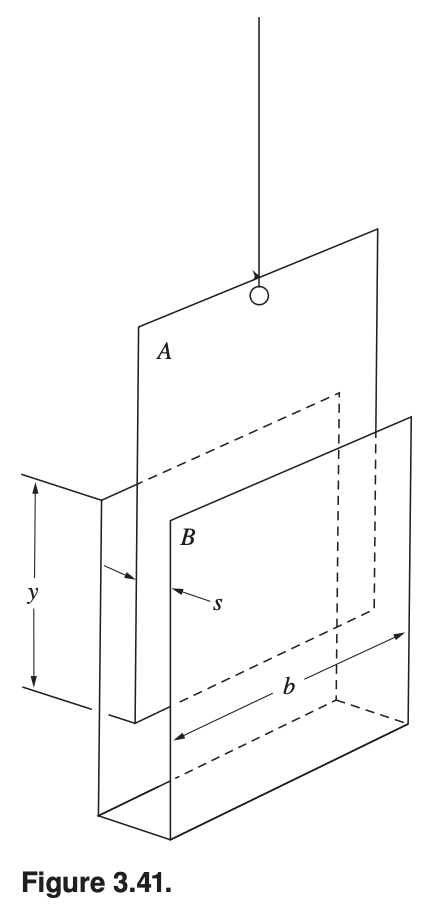
\includegraphics[width=0.3\linewidth]{F3.41.png}
\end{figure}

\vspace{5mm}
\noindent
\textbf{Solution} \, The sheet A form two parallel capacitors with B on both side of the sheet, so the capacitance between the two sheets is
$$C=\frac{\varepsilon_0 A}{s} = \frac{2\varepsilon_0 yb}{s}.$$
Using equation 3.32, the force is
$$F' = \frac{Q^2}{2} \frac{\mathrm{d}}{\mathrm{d}y} \left( \frac{1}{C}\right) = -\frac{C^2V^2}{2} \frac{s}{2\varepsilon_0y^2b}= -\frac{V^2\varepsilon_0b}{s}.$$
By Newton's third law, the force pulling $A$ downward is $F=-F'$. Therefore, 
$$V=\sqrt{\frac{Fs}{\varepsilon_0b}}.$$

\pagebreak

\section{Exercise W5}
\subsection{(4.24) \textit{Mean free time in water}}
An ion in a liquid is so closely surrounded by neutral molecules that one can hardly speak of a “free time” between collisions. Still, it is interesting to see what value of $\tau$ is implied by Eq. (4.23) if we take the observed conductivity of pure water from Table 4.1, and if we use $6 \cdot 10^{19} \ \text{m}^{-3}$ for $N_+$ and $N_-$; see Footnote 4. A typical thermal speed for a water molecule is $500 \ \text{m/s}$. How far would it travel in that time $\tau$?

\vspace{5mm}
\noindent
\textbf{Solution} \, Assuming the conducting ions in pure water are $\text{OH}^-$ and $\text{H}_3\text{O}^+$, we apply Eq. (4.23):
$$\sigma \approx e^2 \cdot 6 \cdot 10^{19} \left( \frac{1}{17\cdot 10^{-3} / N_\mathrm{A}} + \frac{1}{19\cdot 10^{-3} / N_{\mathrm{A}}}\right) \tau = 4 \cdot 10^{-6} \implies \tau = 4 \cdot 10^{-14} \ \text{s}.$$
In the time $\tau$, the travel distance is $d=v\tau = 2\cdot 10^{-11} \ \text{m}$.

\subsection{(4.32) \textit{Tapered rod}}
Two graphite rods are of equal length. One is a cylinder of radius $a$. The other is conical, tapering (or widening) linearly from radius $a$ at one end to radius $b$ at the other. Show that the end-to-end electrical resistance of the conical rod is $a/b$ times that of the cylindrical rod. Hint: Consider the rod to be made up of thin, disk-like slices, all in series. (This result is actually only an approximate one, valid in the limit where the taper is slow. See Problem 4.6 for a discussion of this.)

\vspace{5mm}
\noindent
\textbf{Solution} \, Let the length of the rods be $l$. Then the resistance of the cylindrical rod is $R_1 = \rho l/\pi a^2$. 

For the tapered rod, consider a thin cross-section of the rod with distance $x$ from the base. The resistance of this slice is
$$\mathrm{d}R = \frac{\rho L}{A} = \frac{\rho \, \mathrm{d}x}{\pi (b-(b-a)x/l)^2}.$$
Integrate it over the whole rod, the total resistance is 
$$R_2 = \int _0^l \, \mathrm{d}R = \int_0^l \frac{\rho \, \mathrm{d}x}{\pi (b-(b-a)x/l)^2} =  \frac{\rho l}{\pi ab}.$$
Therefore, $R_2/R_1=a/b$.

\subsection{(4.35) \textit{Resistances in a cube}}
A cube has a resistor $R$ along each edge. Find the equivalent resistance between two nodes that correspond to:\\[3mm]
(a) diagonally opposite corners of the cube;\\
(b) diagonally opposite corners of a face;\\
(c) adjacent corners.\\[3mm]
You do not need to solve a number of simultaneous equations; instead use symmetry arguments. Hint: If two vertices are at the same potential, they can be collapsed to one point without changing the equivalent resistance between the two given nodes.

\vspace{5mm}
\noindent
\textbf{Solution} \, 
\begin{figure}[H]
    \centering
    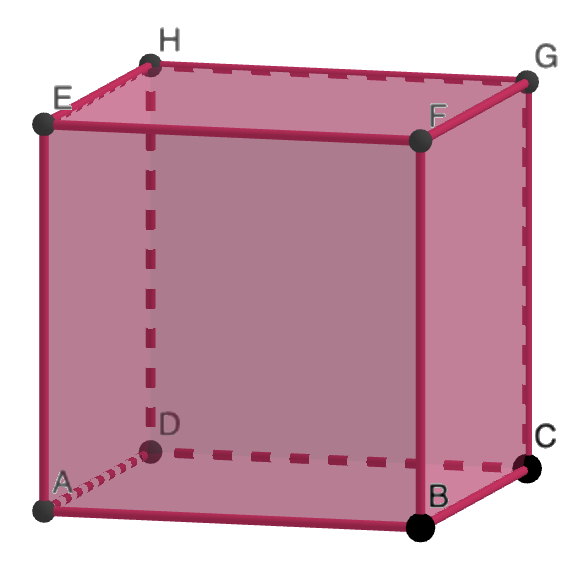
\includegraphics[width=0.3\linewidth]{Q4.35.png}
\end{figure}
\noindent(a) Consider an input voltage between corners $A$ and $G$. Corners $B$, $D$ and $E$ are equipotential, and corners $C$, $F$ and $H$ are equipotential. Collapse two sets of corners, the circuit between $A$ and $G$ is equivalent to:
\begin{center}
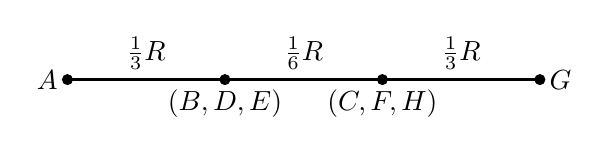
\begin{tikzpicture}
    \draw [thick] (0,0) -- (6,0);

    \fill (0,0) circle (2pt);
    \fill (6,0) circle (2pt);

    \fill (2,0) circle (2pt);
    \fill (4,0) circle (2pt);

    \node[left] at (0,0) {$A$};
    \node[right] at (6,0) {$G$};
    \node[below] at (2,0) {$(B,D,E)$};
    \node[below] at (4,0) {$(C,F,H)$};

    \node[above] at (1,0) {$\frac{1}{3}R$};
    \node[above] at (3,0) {$\frac{1}{6}R$};
    \node[above] at (5,0) {$\frac{1}{3}R$};
\end{tikzpicture}
\end{center}
The equivalent resistance is
$$R_1 = \frac{R}{3}+\frac{R}{6}+\frac{R}{3} = \frac{5R}{6}.$$\\[3mm]
(b) Consider an input voltage between corners $A$ and $C$. Corners $B$, $D$, $F$ and $H$ are equipotential. Collapse this sets of corners, the circuit between $A$ and $C$ is equivalent to:
\begin{center}
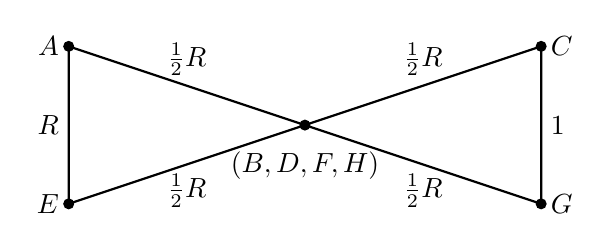
\begin{tikzpicture}
    \coordinate (A) at (0,2);
    \coordinate (B) at (6,2);
    \coordinate (C) at (3,1);
    \coordinate (D) at (0,0);
    \coordinate (E) at (6,0);

    \draw [thick] (A) -- (D) -- (C) -- (B) -- (E) -- (C) -- (A);

    \fill (A) circle (2pt);
    \fill (B) circle (2pt);
    \fill (C) circle (2pt);
    \fill (D) circle (2pt);
    \fill (E) circle (2pt);
    
    \node[left] at (A) {$A$};
    \node[right] at (B) {$C$};
    \node[left] at (D) {$E$};
    \node[right] at (E) {$G$};
    \node[below, yshift = -6pt] at (C) {$(B,D,F,H)$};
    
    \node[left] at (0,1) {$R$};
    \node[right] at (6,1) {$1$};
    \node[above] at (1.5,1.5) {$\frac{1}{2}R$};
    \node[above] at (4.5,1.5) {$\frac{1}{2}R$};
    \node[below] at (1.5,0.5) {$\frac{1}{2}R$};
    \node[below] at (4.5,0.5) {$\frac{1}{2}R$};
\end{tikzpicture}
\end{center}
The equivalent resistance is
$$R_2 = \frac{1}{\frac{1}{R+R/2}+\frac{1}{R/2}}+\frac{1}{\frac{1}{R+R/2}+\frac{1}{R/2}} = \frac{3R}{4}.$$\\[3mm]
(c) Consider an input voltage between corners $A$ and $B$. Corners $D$ and $E$ are equipotential, and corners $C$ and $F$ are equipotential. Collapse two pairs of corners, the circuit between $A$ and $B$ is equivalent to:
\begin{center}
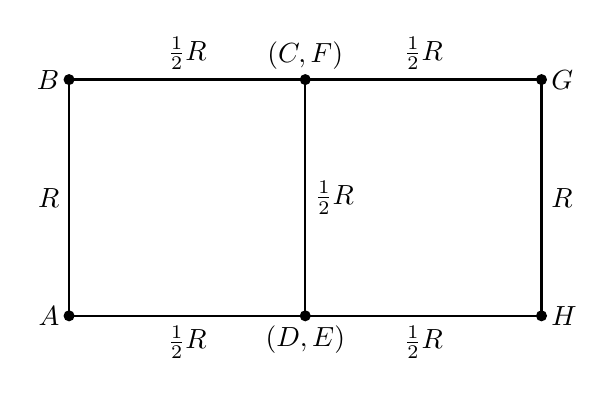
\begin{tikzpicture}
    \coordinate (A) at (0,0);
    \coordinate (B) at (0,3);
    \coordinate (C) at (3,0);
    \coordinate (D) at (3,3);
    \coordinate (E) at (6,0);
    \coordinate (F) at (6,3);

    \draw [thick] (A) -- (B) -- (D) -- (C) -- (A);
    \draw [thick] (D) -- (F) -- (E) -- (C);

    \fill (A) circle (2pt);
    \fill (B) circle (2pt);
    \fill (C) circle (2pt);
    \fill (D) circle (2pt);
    \fill (E) circle (2pt);
    \fill (F) circle (2pt);

    \node[left] at (A) {$A$};
    \node[left] at (B) {$B$};
    \node[below] at (C) {$(D,E)$};
    \node[above] at (D) {$(C,F)$};
    \node[right] at (E) {$H$};
    \node[right] at (F) {$G$};

    \node[left] at (0,1.5) {$R$};
    \node[below] at (1.5,0) {$\frac{1}{2}R$};
    \node[below] at (4.5,0) {$\frac{1}{2}R$};  
    \node[above] at (1.5,3) {$\frac{1}{2}R$};
    \node[above] at (4.5,3) {$\frac{1}{2}R$};
    \node[right] at (3,1.5) {$\frac{1}{2}R$};
    \node[right] at (6,1.5) {$R$};
\end{tikzpicture}
\end{center}
The equivalent resistance is
$$\frac{1}{R_3} = \frac{1}{R} + \frac{1}{\frac{R}{2}+ \frac{1}{2/R+1/2R} +\frac{R}{2}  } \implies R_3 = \frac{7R}{12}.$$

\subsection{(4.36) \textit{Attenuator chain}}
Some important kinds of networks are infinite in extent. Figure 4.49 shows a chain of series and parallel resistors stretching off endlessly to the right. The line at the bottom is the resistanceless return wire for all of them. This is sometimes called an attenuator chain, or a ladder network. 

The problem is to find the “input resistance,” that is, the equivalent resistance between terminals $A$ and $B$. Our interest in this problem mainly concerns the method of solution, which takes an odd twist and which can be used in other places in physics where we have an iteration of identical devices (even an infinite chain of lenses, in optics). The point is that the input resistance (which we do not yet know – call it $R$) will not be changed by adding a new set of resistors to the front end of the chain to make it one unit longer. But now, adding this section, we see that this new input resistance is just $R_1$ in series with the parallel combination of $R_2$ and $R$.

Use this strategy to determine $R$. Show that, if voltage $V_0$ is applied at the input to such a chain, the voltage at successive nodes decreases in a geometric series. What should the ratio of the resistors be so that the ladder is an attenuator that halves the voltage at every step? Obviously a truly infinite ladder would not be practical. Can you suggest a way to terminate it after a few sections without introducing any error in its attenuation?
\begin{figure}[H]
    \centering
    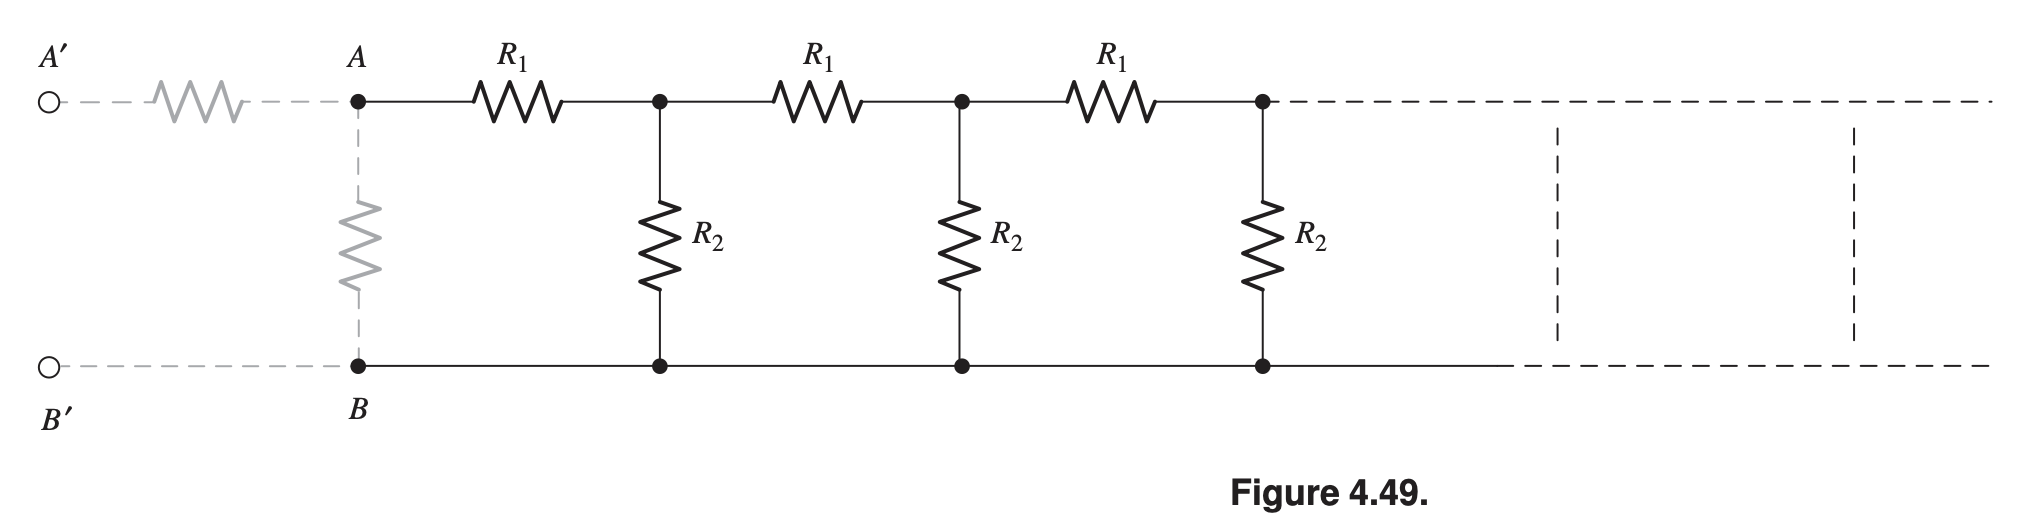
\includegraphics[width=1\linewidth]{F4.49.png}
\end{figure}

\vspace{5mm}
\noindent
\textbf{Solution} \, The circuit is equivalent to
\begin{center}
\begin{circuitikz}
    \draw[line width=1pt] (0,0) node[above] {$A'$} to[short, o-] (0.01,0);
    \draw[line width=1pt] (0.05,0) to[R=$R_1$] (3,0) node[above] {$A$};
    \draw[line width=1pt] (3,0)  to[R=$R_2$] (3,-3);
    \draw[line width=1pt] (3,0) to[short] (5,0);
    \draw[line width=1pt] (5,0) to[R=$R$] (5,-3);
    \draw[line width=1pt] (3,-3) to[short] (5,-3);
    \draw[line width=1pt] (0,-3) node[below] {$B'$} to[short, o-] (3,-3) node[below] {$B$};
    \draw[line width=1pt, stealth-stealth] (0,-0.1) -- (0,-2.9) node[midway, left] {$R$};
    \fill (3,0) circle (2pt);
    \fill (3,-3) circle (2pt);
\end{circuitikz}
\end{center}
Therefore,
$$R = R_1 + \frac{1}{\frac{1}{R}+\frac{1}{R_2}} \implies R^2-R_1R-R_1R_2=0 \implies R = \frac{R_1+\sqrt{R_1^2+4R_1R_2}}{2}.$$

Consider an input voltage $V'$ between $A'$ and $B'$. The total current through the circuit right to the input is $V'/R$, so the voltage between $A$ and $B$ is $V=V'-V'R_1/R$. Therefore, the voltage decreases by ratio
$$\frac{V}{V'}=\frac{V'-V'R_1/R}{V'} = \frac{R-R_1}{R}.$$
This holds for any adjacent nodes in the chain, so the voltage at successive nodes decreases in a geometric series.

If the attenuator halves the voltage each step, then
$$\frac{R-R_1}{R}=\frac{1}{2} \implies R=\frac{R_1+\sqrt{R_1^2+4R_1R_2}}{2} = 2R_1 \implies R_2=2R_1.$$

To terminate the ladder after a few section without introducing any error in its attenuation, simply replace the rest infinite chain with a resistor $R$ given, just like the equivalent circuit above shown.

\subsection{(4.45) \textit{Battery/resistor loop}}
In the circuit shown in Fig. 4.57, all five resistors have the same value, $100$ ohms, and each cell has an electromotive force of $1.5$ V. Find the open-circuit voltage and the short-circuit current for the terminals $A$ and $B$. Then find $\varepsilon_{eq}$ and $R_{eq}$ for the Thévenin equivalent circuit.
\begin{figure}[H]
    \centering
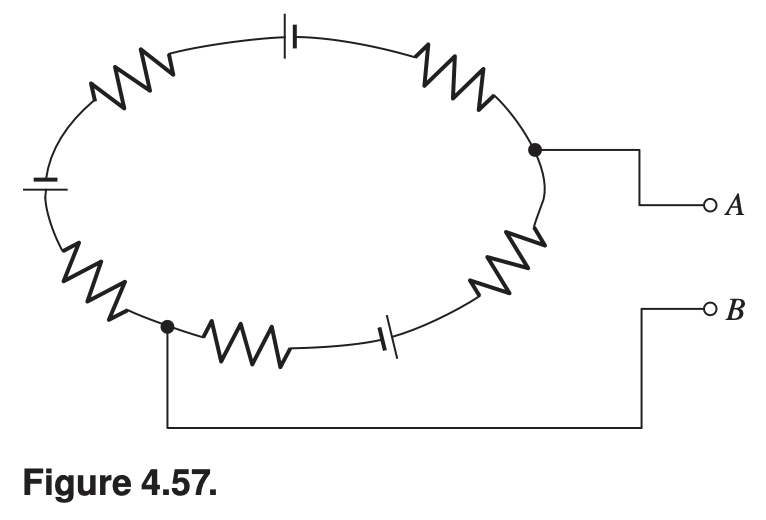
\includegraphics[width=0.45\linewidth]{F4.57.png}
\end{figure}

\vspace{5mm}
\noindent
\textbf{Solution} \, Let the circuit be open first. Then inside the loop, the current is
$$I = \frac{3E}{5R} = \frac{3\cdot 1.5 \ \text{V}}{5\cdot 100 \ \text{ohm}} = 9\cdot 10^{-3} \ \text{A}.$$
Therefore, the open-circuit voltage is
$$V_{BA} = -E+2IR = -1.5\ \text{V} + 2\cdot 9\cdot 10^{-3} \ \text{A} \cdot 100 \ \text{ohm} = 0.3 \ \text{V}.$$

Then connect $A$ and $B$. The circuit is equivalent to 
\begin{center}
\begin{circuitikz}[line width = 1pt]
    \draw (0,0) node[above] {$A$} to (0,-3) node[below] {$B$};
    \draw (0,0) to[R, l_=3R] (-3,0) to[battery, invert, l_=$2E$] (-3, -3) to (0,-3);
    \draw (0,0) to (3,0) to[battery, l=$E$] (3,-3) to[R=$2R$] (0,-3);

    \fill (0,0) circle (2pt);
    \fill (0,-3) circle (2pt);

    \draw[->] (-0.8, -1.5) arc[start angle=0,end angle=350,radius=0.7];
    \node at (-1.5, -1.5) {$I_1$};
    \draw[->] (2.2, -1.5) arc[start angle=0,end angle=350,radius=0.7];
    \node at (1.5, -1.5) {$I_2$};
\end{circuitikz}
\end{center}
Therefore, the short-circuit current is
$$I_{BA} = I_1 - I_2 = \frac{2E}{3R} - \frac{E}{2R} = \frac{E}{6R} = 2.5 \cdot 10^{-3} \ \text{A}.$$

In the Thévenin equivalent circuit,
$$\varepsilon_{eq} = V_{BA} = 0.3 \ \text{V}, \ R_{eq} = \frac{\varepsilon_{eq}}{I_{BA}} = 120 \ \text{ohm}.$$

\subsection{(4.48) \textit{Charging a capacitor}}
Problem 4.17 deals with the charging of a capacitor. Using the results from that problem, show that energy is conserved. That is, show that the total work done by the battery equals the final energy stored in the capacitor plus the energy dissipated in the resistor.

\vspace{5mm}
\noindent
\textbf{Solution} \, The total work done by the battery is $W=EQ$, where $E$ is the emf of the battery and $Q$ is the final charge on the capacitor. The final energy of the capacitor is $E_C = EQ/2$. The energy dissipated in the resistor is
$$E_R = \int_0^\infty I^2R \, \mathrm{d}t = \int_0^\infty (\frac{E}{R}e^{-t/RC})^2R \, \mathrm{d}t = \frac{CE^2}{2} = \frac{EQ}{2}.$$
Therefore,
$$W = EQ = E_C + E_R.$$
The energy is indeed conserved.

\pagebreak

\section{Exercise W6}
\subsection{(5.12) \textit{Tilted sheet}}
Redo the “Tilted sheet” example in Section 5.5 in terms of a general $\gamma$ factor, to verify that Gauss’s law holds for any choice of the relative speed of the two frames.

\vspace{5mm}
\noindent
\textbf{Solution} \, In going from $F$ to $F'$, longitudinal distances are decreased by $1/ \gamma$, so
$$\sigma \cdot \sqrt{2}l = \sigma' \cdot \sqrt{1+\left( \frac{1}{\gamma}\right)^2} l \implies \sigma' = \frac{\sqrt{2}\gamma}{\sqrt{1+\gamma^2}}\sigma.$$

The magnitude of the field $\vb{E}$ in $F$ is $E= \sigma/2\varepsilon_0$, so the field component in $F'$ is
$$E_\perp' = \gamma E_\perp = \frac{\gamma E}{\sqrt{2}}, \quad E_\parallel' = E_\parallel = \frac{E}{\sqrt{2}}. $$
Therefore, the field in $F'$ has magnitude
$$E' = \sqrt{E_\perp'^2+E_\parallel'^2} = \sqrt{\frac{\gamma^2E^2}{2}+\frac{E^2}{2}} = \frac{\sqrt{1+\gamma^2}E}{\sqrt{2}},$$
and it points at an angle of $2\arctan \gamma-\pi/4$ with respect to the normal to
the sheet, so the normal component of $E'$ is
$$E'_n = E' \cos (2\arctan \gamma - \frac{\pi}{4}) = E' \cdot 2\sin (\arctan \gamma) \cos (\arctan \gamma) = \frac{\sqrt{1+\gamma^2}E}{\sqrt{2}} \cdot \frac{2\gamma}{1+\gamma^2} = \frac{\sqrt{2} \gamma}{\sqrt{1+\gamma^2}}E.$$
$E'_n$ has the same factor to $E$ with that of $\sigma'$ to $\sigma$, so Gauss's law still holds in $F'$. 

\subsection{(5.13) \textit{Adding the fields}}
A stationary proton is located on the $z$ axis at $z = a$. A negative muon is moving with speed $0.8c$ along the $x$ axis. Consider the total electric field of these two particles, in this frame, at the time when the muon passes through the origin. What are the values at that instant of $E_x$ and $E_z$ at the point $(a, 0, 0)$ on the $x$ axis?

\vspace{5mm}
\noindent
\textbf{Solution} \, For the field due to the proton,
$$E_{px} = \frac{1}{2\sqrt{2}} \cdot  \frac{e}{4\pi \varepsilon_0 a^2}, \quad E_{pz} = -\frac{1}{2\sqrt{2}} \cdot \frac{e}{4\pi \varepsilon_0 a^2}.$$
For the field due to the muon,
$$E_{\mu x} = -\frac{e}{4\pi \varepsilon_0 a'^2} = -\frac{e}{4\pi \varepsilon_0 \left(\gamma a\right)^2} = -\left(1-\frac{v^2}{c^2}\right) \cdot \frac{e}{4\pi \varepsilon_0 a^2} = -0.36 \frac{e}{4\pi \varepsilon_0 a^2}.$$
Add them up,
$$E_x = \left(\frac{1}{2\sqrt{2}}-0.36\right) \cdot \frac{e}{4\pi \varepsilon_0 a^2}, \quad E_z = \frac{1}{2\sqrt{2}} \cdot \frac{e}{4\pi \varepsilon_0 a^2}.$$

\subsection{(5.15) \textit{Gauss’s law for a moving charge}}
Verify that Gauss’s law holds for the electric field in Eq. (5.15). That is, verify that the flux of the field, through a sphere centered at the charge, is $q/\varepsilon_0$. Of course, we used this fact in deriving Eq. (5.15) in the first place, so we know that it must be true. But it can’t hurt to double check. You’ll want to use a computer or the integral table in Appendix K.

\vspace{5mm}
\noindent
\textbf{Solution} \, Consider a sphere enclosing a single moving charge. Calculate the total flux by integrating over every slice of the sphere perpendicular to the moving direction:
\begin{align}
   \int_S E \, \mathrm{d}a &= \int_0^\pi \frac{Q}{4\pi \varepsilon_0 r^2} \cdot \frac{1-\beta^2}{(1-\beta^2 \sin ^2 \theta)^{3/2}} \cdot 2\pi r \sin \theta \cdot r\, \mathrm{d}\theta \\
   &=\frac{Q(1-\beta^2)}{2\varepsilon_0} \int_0^\pi \frac{\sin \theta}{(1-\beta^2 \sin^2 \theta)^{3/2}}\, \mathrm{d}\theta \\ 
   & = \frac{Q(1-\beta^2)}{2\varepsilon_0} \cdot \frac{\cos \theta}{(\beta^2-1)\sqrt{1-\beta^2 \sin ^2 \theta}} \Bigg|_0^\pi \\
   & = \frac{Q(1-\beta^2)}{2\varepsilon_0} \cdot \frac{2}{1-\beta^2}\\
   & = \frac{Q}{2\varepsilon_0}.
\end{align}
This is exactly Gauss's law.

\subsection{(5.24) \textit{Acquiring transverse momentum}}
In the rest frame of a particle with charge $q_1$, another particle with charge $q_2$ is approaching, moving with velocity $v$ not small compared with $c$. If it continues to move in a straight line, it will pass a distance $b$ from the position of the first particle. It is so massive that its displacement from the straight path during the encounter is small compared with $b$. Likewise, the first particle is so massive that its displacement from its initial position while the other particle is nearby is also small compared with $b$.\\[3mm]
(a) Show that the increment in momentum acquired by each particle as a result of the encounter is perpendicular to $\vb{v}$ and has magnitude $q_1 q_2/2\pi \varepsilon_0 vb$. (Gauss’s law can be useful here.)\\
(b) Expressed in terms of the other quantities, how large (in order of magnitude) must the masses of the particles be to justify our assumptions?

\vspace{5mm}
\noindent
\textbf{Solution} \, (a) Let $q_2$ be moving along the $x$ axis, and $q_1$ be placed on $y$ axis. The momentum acquired by $q_1$ equals to the integral of force applied by $q_2$ over time $t$, so by symmetry, the momentum on $x$ axis is zero, and the total momentum is along $y$ axis, i.e. perpendicular to to $\vb{v}$. 
$$\Delta P_1 = \int q_1E_y \, \mathrm{d}t =\frac{q_1}{v} \int_{-\infty}^{+\infty} E_y \, \mathrm{d}x.$$
By Gauss's law, one can tell that, through the surface of an infinitely long cylinder with a radius $b$, the total flux due to one point charge $q_2$ is
$$\int_{-\infty}^{+\infty} E\cdot 2\pi b \, \mathrm{d}x = \frac{q_2}{\varepsilon_0} \implies \int_{-\infty}^{\infty}E\, \mathrm{d}x = \frac{q_2}{2\pi b \varepsilon_0}.$$
Therefore, 
$$\Delta P_1 = \frac{q_1}{v} \int_{-\infty}^{+\infty} E_y \, \mathrm{d}x = \frac{q_1q_2}{2\pi \varepsilon_0 vb}.$$
By Newton’s third law, the momentum acquired by $q_1$ is equal and opposite to
the momentum acquired by $q_2$, so $\Delta P_2 = q_1q_2/2\pi \varepsilon_0 vb$ and is perpendicular to $\vb{v}$. \\[3mm]
(b) Our assumptions were that the particles are so massive that during the encounter their trajectories deviate only slightly from a straight line. In other words, the impulse $\Delta P_2$ must be small compared with the initial momentum. Therefore,
$$\gamma m_2v \gg \Delta P_2 = \frac{q_1q_2}{2\pi \varepsilon_0 v b} \implies m_2 \gg \frac{q_1q_2}{2\pi\varepsilon_0 \gamma v^2 b}.$$
Since $q_1$ and $q_2$ are essentially equivalent by changing the frame, $m_1$ should be at the same magnitutde. Therefore, $m_1$ and $m_2$ must satisfy:
$$m \gg \frac{q_1q_2}{2\pi\varepsilon_0 \gamma v^2 b}.$$

\pagebreak

\section{Exercise W7}
\subsection{(5.28) \textit{Stationary rod and moving charge}}
A charge $q$ moves with speed $v$ parallel to a long rod with linear charge density $\lambda$, as shown in Fig. 5.30. The rod is at rest. If the charge $q$ is a distance $r$ from the rod, the force on it is simply $F= qE= q\lambda/2\pi r \varepsilon_0$. 

Now consider the setup in the frame that moves along with the charge $q$. What is the force on the charge $q$ in this new frame? Solve this by:\\[3mm]
(a) transforming the force from the old frame to the new frame, without caring about what causes the force in the new frame; \\
(b) calculating the electric force in the new frame.
\begin{figure}[H]
    \centering
    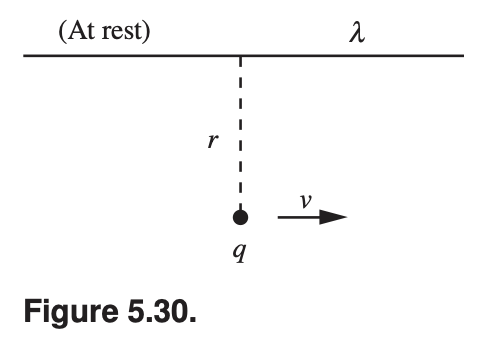
\includegraphics[width=0.3\linewidth]{F5.30.png}
\end{figure}

\vspace{5mm}
\noindent
\textbf{Solution} \, (a) By transforming the frame, $E_\perp'=\gamma E_\perp$. Therefore the force in the new frame is
$$F' = E_\perp'q = \frac{\gamma q \lambda}{2\pi r \varepsilon_0}.$$ \\[3mm]
(b) In the frame of $q$, the charge density of the rod is enlarged to $\gamma \lambda$ due to length contraction. Therefore the electric force is
$$F' = \frac{q\gamma \lambda}{2\pi r \varepsilon_0}.$$

\subsection{(5.30) \textit{Transformations of $\boldsymbol{\lambda}$ and $\boldsymbol{I}$}}
Consider a composite line charge consisting of several kinds of carriers, each with its own velocity. For each kind, labeled by $k$, the linear density of charge measured in frame $F$ is $\lambda_k$, and the velocity is $\beta_kc$ parallel to the line. The contribution of these carriers to the current in $F$ is then $I_k = \lambda_k \beta_k c$. How much do these $k$-type carriers contribute to the charge and current in a frame $F'$ that is moving parallel to the line at velocity $-\beta c$ with respect to $F$? By following the steps we took in the transformations in Fig. 5.22, you should be able to show that
$$\lambda_k' = \gamma\left(\lambda_k + \frac{\beta I_k}{c}\right), \quad I_k' = \gamma(I_k + \beta c \lambda_k).$$
If each component of the linear charge density and current transforms in this way, then so must the total $\gamma$ and $I$:
$$\lambda' = \gamma\left(\lambda + \frac{\beta I}{c}\right), \quad I' = \gamma(I + \beta c \lambda).$$
You have now derived the Lorentz transformation to a parallel-moving frame for \textit{any} line charge and current, whatever its composition.

\vspace{5mm}
\noindent
\textbf{Solution} \, Based on the derivation in Fig. 5.22, the speed of charges in the new frame $F'$ should follow
$$\beta_k' = \frac{\beta_k + \beta}{1+\beta \beta_k}, \quad \gamma_k' = \gamma \gamma_k(1+\beta \beta_k).$$
Therefore, in frame $F'$,
$$\lambda_k' = \lambda_k \frac{\gamma_k'}{\gamma_k} = \lambda_k \gamma (1+\beta \beta_k) = \gamma \left(\lambda_k+ \beta \lambda_k \beta_k\right) = \gamma\left(\lambda_k + \frac{\beta I_k}{c}\right),$$
and 
$$I_k' = \lambda_k' \beta_k' c = \lambda_k \gamma (1+\beta \beta_k) \cdot \frac{\beta_k + \beta}{1+\beta \beta_k} \cdot c = \gamma(I_k+ \beta c \lambda_k).$$
Such transformations are linear, and since the total charge density $\lambda$ and current $I$ are both linear combinations of the $\lambda_k$ and $I_k$, the transformations above also apply to $\lambda$ and $I$.

\subsection{(6.38) \textit{Uniform field in off-center hole}}
A cylindrical rod with radius $R$ carries current $I$ (with uniform current density), with its axis lying along the $z$ axis. A cylindrical cavity with an arbitrary radius is hollowed out from the rod at an arbitrary location; a cross section is shown in Fig. 6.44. Assume that the current density in the remaining part stays the same (which would be the case for a fixed voltage difference between the ends). Let $\vb{a}$ be the position of the center of the cavity with respect to the center of the rod. Show that the magnetic field inside the cylindrical cavity is uniform (in both magnitude and direction). Hint: Show that the field inside a solid cylinder can be written in the form $\vb{B}= (\mu_0 I/2\pi R^2) \vu{z} \times \vb{r}$, and then use superposition with another appropriately chosen cylinder.
\begin{figure}[H]
    \centering
    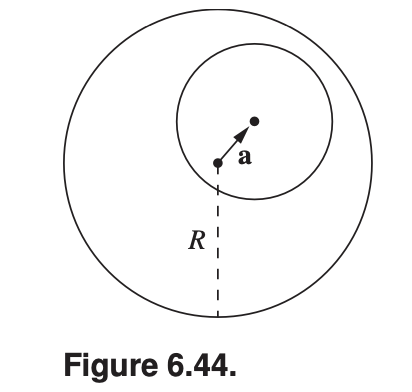
\includegraphics[width=0.3\linewidth]{F6.44.png}
\end{figure}

\vspace{5mm}
\noindent
\textbf{Solution} \, Inside a rod without any cavities, the current enclosed by a circle of radius $r$ is $I_r = Ir^2/R^2$. Based on Ampère's law,
$$B \cdot 2\pi r = \mu_0  \frac{Ir^2}{R^2} \implies B = \frac{\mu_0 Ir}{2\pi R^2}.$$
The direction of the magnetic field is tangential $\vu{\boldsymbol{\theta}} = \vu{z} \times \vu{r}$, so the field inside the solid cylinder can be written as
$$\vb{B} = \frac{\mu_0Ir}{2\pi R^2}\vu{z} \times \vu{r} = \frac{\mu_0I}{2\pi R^2}\vu{z}\times \vb{r}.$$

Now consider an arbitrary point inside the cavity, at $\vb{r}_1$ and $\vb{r}_2$ with respect to the center of the rod and the center of the cavity, respectively. The magnetic field at the point is a superposition of the solid rod and a negative current inside the cavity, which is
$$\vb{B} = \frac{\mu_0I_R}{2\pi R^2}\vu{z}\times \vb{r}_1 - \frac{\mu_0I_r}{2\pi r^2}\vu{z}\times \vb{r_2},$$
where $I_r$ and $r$ denote the current and radius of the cavity. Since the current density is fixed,
$$J = \frac{I_R}{\pi R^2} = \frac{I_r}{\pi r^2}.$$
Therefore,
$$\vb{B} = \frac{1}{2}\mu_0 J\vu{z}\times \vb{r}_1 - \frac{1}{2}\mu_0 J\vu{z}\times \vb{r}_2 = \frac{1}{2}\mu_0 J \vu{z} \times (\vb{r}_1 - \vb{r}_2) = \frac{1}{2}\mu_0 J \vu{z} \times \vb{a},$$
which is uniform in both magnitude and direction.

\subsection{(6.43) \textit{Vector potential inside a wire}}
A round wire of radius $r_0$ carries a current $I$ distributed uniformly over the cross section of the wire. Let the axis of the wire be the $z$ axis, with $\vu{z}$ the direction of the current. Show that a vector potential of the form $\vb{A} = A_0 \vu{z} (x^2 +y^2)$ will correctly give the magnetic field $\vb{B}$ of this current at all points inside the wire. What is the value of the constant, $A_0$?

\vspace{5mm}
\noindent
\textbf{Solution} \, Applying Ampère's law, the magnetic field at radius $r$ has magnitude
$$B(r) \cdot 2\pi r = \mu_0 I \frac{r^2}{r_0^2} \implies B(r) = \frac{\mu_0 I r}{2\pi r_0^2}$$
and tangential direction. So $\vb{B} = (\mu_0Ir/2\pi r_0^2)\vu{\boldsymbol{\theta}}$. On the other hand, $\vb{A} = A_0 r^2 \vu{z}$. Therefore,
$$\vb{B} = \curl{\vb{A}} = -(\frac{\partial A_z}{\partial r})\vu{\boldsymbol{\theta}} = -2A_0 r \vu{\boldsymbol{\theta}}.$$
Compare the two expressions:
$$A_0 = -\frac{\mu_0 I}{4\pi r_0^2}.$$ 

\subsection{(6.46) \textit{Field from a wire frame}}
(a) Current $I$ flows around the wire frame in Fig. 6.45(a). What is the direction of the magnetic field at $P$, the center of the cube? \\
(b) Show by using superposition that the field at $P$ is the same as if the frame were replaced by the single square loop shown in Fig. 6.45(b).
\begin{figure}[h]
    \centering
    \begin{minipage}{0.4\textwidth}
        \centering
        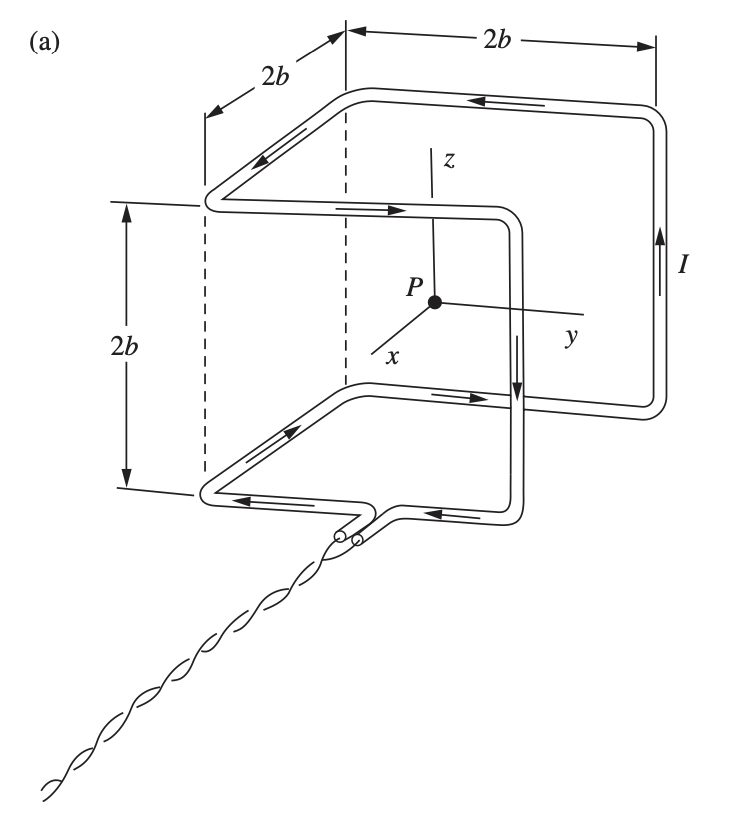
\includegraphics[width=\textwidth]{F6.45(a).png}
    \end{minipage}
    \begin{minipage}{0.4\textwidth}
        \centering
        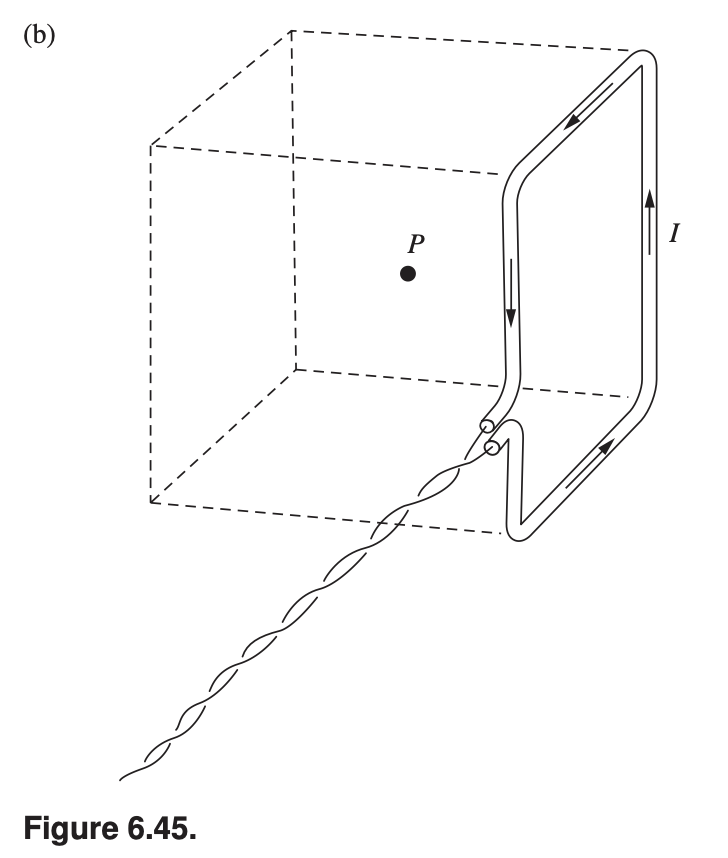
\includegraphics[width=\textwidth]{F6.45(b).png}
    \end{minipage}
\end{figure}

\vspace{5mm}
\noindent
\textbf{Solution} \, (a) The current in the upper and lower planes of the cube each generates a magnetic field at $P$ with same magnitude but with opposite direction, so they cancel out. The current of the two vertical edges each generates a magnetic field at $P$ with same positive $y$ component and opposite $x$ component. Therefore, the magnetic field at $P$ points in the positive $y$ direction.\\[3mm]
(b) Imagine a clockwise (view from $+z$) circuit $I$ on the upper plane, and a counterclockwise circuit $I$ on the lower plane. Such two currents each would generate a magnetic field at $P$ with same magnitude and opposite direction, so they would cancel out. Superimpose the two current on the wire frame, and the result is exactly the same as in Fig. 6.45(b), while the magnetic field at $P$ is unchanged.

\pagebreak

\section{Exercise 8}
\subsection{\textit{Magnetic Field in a cylinder}}
An infinitely long cylindrical shell of radius $R$ carrying a uniform surface current $\vb{J}$ produces a strictly uniform axial field $B_z$ inside. Proof it in two ways:\\[3mm]
(a) Calculate the vector potential $\vb{A}$ due to $\vb{J}$.\\
(b) Use Bivot-Savart law.

\vspace{5mm}
\noindent
\textbf{Solution} \, (a) By symmetry $\vb{A}$ can only have an azimuthal component: $\vb{A} = A_\phi(r)\,\vu{phi}$. In cylindrical coordinates, the $\phi$–component of $\laplacian{\vb{A}}$ is
$$(\laplacian{\vb{A}})_{\phi} = \frac{1}{r}\frac{\mathrm{d}}{\mathrm{d}r}\left(r\,\frac{\mathrm{d}A_\phi}{\mathrm{d}r}\right) - \frac{A_\phi}{r^2}.$$
Therefore,
$$\frac{1}{r}\frac{\mathrm{d}}{\mathrm{d}r}\left(r\,\frac{\mathrm{d}A_\phi}{\mathrm{d}r}\right) - \frac{A_\phi}{r^2} = -\mu_0 \vb{J}.$$
This solves for $A_{\phi}(r) = \mu_0 Jr/2 $ within the cylinder. So the magnetic field inside is
$$\vb{B} = \curl{\vb{A}} = \frac{1}{r} \frac{\mathrm{d}}{\mathrm{d}r}\left(rA_\phi\right)\vu{z} = \mu_0J\vu{z},$$
which is uniform inside the shell. \\[3mm]
(b) Consider the contribution of every ring current with polar angle $\phi$.
$$\mathrm{d}B(\phi)= (\mathrm{d}I)\frac{\mu_0 R^2}{2r^3} = \left(\frac{Jr\,\mathrm{d}\phi}{\sin \phi} \right)\frac{\mu_0 R^2}{2r^3}=  \frac{\mu_0 J}{2} \sin \phi \, \mathrm{d}\phi.$$
Integrate it over the whole cylindrical shell, the field strength is
$$B = \frac{\mu_0J}{2} \int_0^\pi \mathrm{d}B = \mu_0 J,$$
and since the field should only have vertical element due to the symmetry,
$$\vb{B} = \mu_0J \vu{z}.$$

\pagebreak

\section{Exercise 9}
\subsection{(6.69) \textit{Relating the forces}}
Two very long sticks each have uniform linear proper charge density $\lambda$. (“Proper” means as measured in the rest frame of the given object.) One stick is stationary in the lab frame, while the other stick moves to the left with speed $v$, as shown in Fig. 6.51. They are $2r$ apart, and a stationary point charge $q$ lies midway between them. Find the electric and magnetic forces on the charge $q$ in the lab frame, and also in the frame of the bottom stick. (Be sure to specify the directions.) Then verify that the total forces in the two frames relate properly.
\begin{figure}[H]
    \centering
    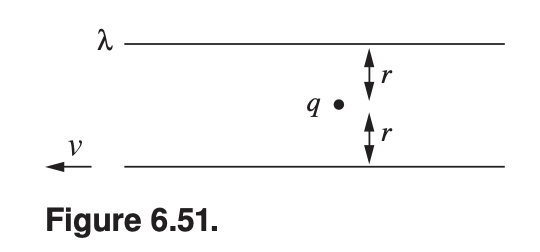
\includegraphics[width=0.3\linewidth]{F6.51.png}
\end{figure}

\vspace{5mm}
\noindent
\textbf{Solution} \, In the lab frame, the charge is at rest, so there is no magnetic force on it. The electric field due to the top stick is $E_1=\lambda/2\pi \varepsilon_0 r$ downward, and the electric field due to the bottom stick is $E_2 = \gamma \lambda/2\pi \varepsilon_0 r$ upward. Therefore the total force on the charge is
$$F = (E_2-E_1)q = (\gamma-1)\frac{\lambda q}{2\pi \varepsilon_0 r}$$
and points upward.

In the frame of the bottom stick, the point charge and the top stick are moving in $v$. The top stick then produces a current of $\gamma \lambda v$, and thus a magnetic field of $\mu_0 \gamma\lambda v/2\pi r$ that points into the paper. The magnetic force on the charge $q$ is therefore $F'_B = qvB = q\mu_0 \gamma\lambda v^2/2\pi r $ and points upward. On the other hand, the electric forces, by similar fashion in the lab frame, is $F'_E = (\gamma-1)\lambda q/2\pi \varepsilon_0 r$ and points downward. The total force in the frame of the bottom stick is
\begin{align*}
    F' & = F'_B-F'_E \\ 
       & = \frac{q\mu_0\gamma \lambda v^2}{2\pi r} - (\gamma-1) \frac{\lambda q}{2\pi \varepsilon_0 r} \\
       & = \frac{\lambda q}{2\pi \varepsilon r} \left( \frac{\gamma v^2}{c^2} - \gamma +1\right) \\
       & = \frac{\lambda q}{2 \pi \varepsilon r} \left( 1-\frac{1}{\gamma}\right)
\end{align*}
and points upward.

The force on the charge in the lab frame is indeed larger than the the force in a moving frame by the factor $\gamma$.

\subsection{(7.26) \textit{Sliding bar}}
A metal crossbar of mass $m$ slides without friction on two long parallel conducting rails a distance $b$ apart; see Fig. 7.35. A resistor $R$ is connected across the rails at one end; compared with $R$, the resistance of bar and rails is negligible. There is a uniform field $B$
perpendicular to the plane of the figure. At time $t = 0$ the crossbar is given a velocity $v_0$ toward the right. What happens afterward?\\[3mm]
(a) Does the rod ever stop moving? If so, when?\\
(b) How far does it go?\\
(c) How about conservation of energy?
\begin{figure}[H]
    \centering
    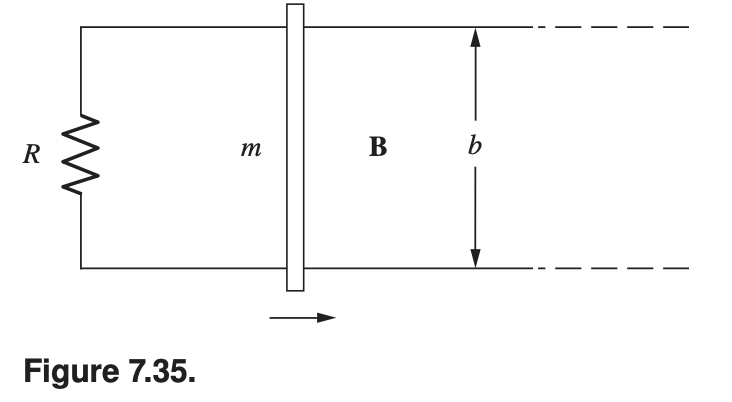
\includegraphics[width=0.4\linewidth]{F7.35.png}
\end{figure}

\vspace{5mm}
\noindent
\textbf{Solution} \, (a) Let $v$ be the velocity of the bar at some $t$. Its movement induces an emf in the circuit, which generates a current that experiences magnetic force in the field. Therefore:
$$F=BIb = Bb\frac{E}{R} = Bb\frac{Bbv}{R} = \frac{B^2b^2v}{R} = -m\frac{\mathrm{d}v}{\mathrm{d}t}.$$
At $t=0$, $v=v_0$. So the equation solves for
$$v=v_0 e^{-\frac{B^2b^2}{mR}t}.$$
The velocity decreases exponentially, so the bar will never stop.\\[3mm]
(b) The total distance the bar traveled in time $t\to \infty$ is
$$x=\int_0^{+\infty} v\, \mathrm{d}t =\int_0^{+\infty} v_0 e^{-\frac{B^2b^2}{mR}t} \, \mathrm{d}t =\frac{v_0mR}{B^2b^2}.$$\\
(c) The initial kinetic energy of the bar is $E_k = mv_0^2/2$. The total heat dissipated by the resistor is
$$Q = \int_0^{+\infty} I^2R \, \mathrm{d}t = \frac{B^2b^2v_0^2}{R} \int_0^{+\infty} e^{-\frac{2B^2b^2}{mR}t} = \frac{B^2b^2v_0^2}{R} \cdot \frac{mR}{2B^2b^2} = \frac{mv_0^2}{2},$$
which indeed equals to $E_k$.

\subsection{(7.27) \textit{Ring in a solenoid}}
An infinite solenoid with radius $b$ has $n$ turns per unit length. The current varies in time according to $I(t)= I_0 \cos{\omega t}$ (with positive defined as shown in Fig. 7.36). A ring with radius $r < b$ and resistance $R$ is centered on the solenoid’s axis, with its plane perpendicular to the axis.\\[3mm]
(a) What is the induced current in the ring?\\
(b) A given little piece of the ring will feel a magnetic force. For what values of t is this force maximum?\\
(c) What is the effect of the force on the ring? That is, does the force cause the ring to translate, spin, flip over, stretch/shrink, etc.?\\
\begin{figure}[H]
    \centering
    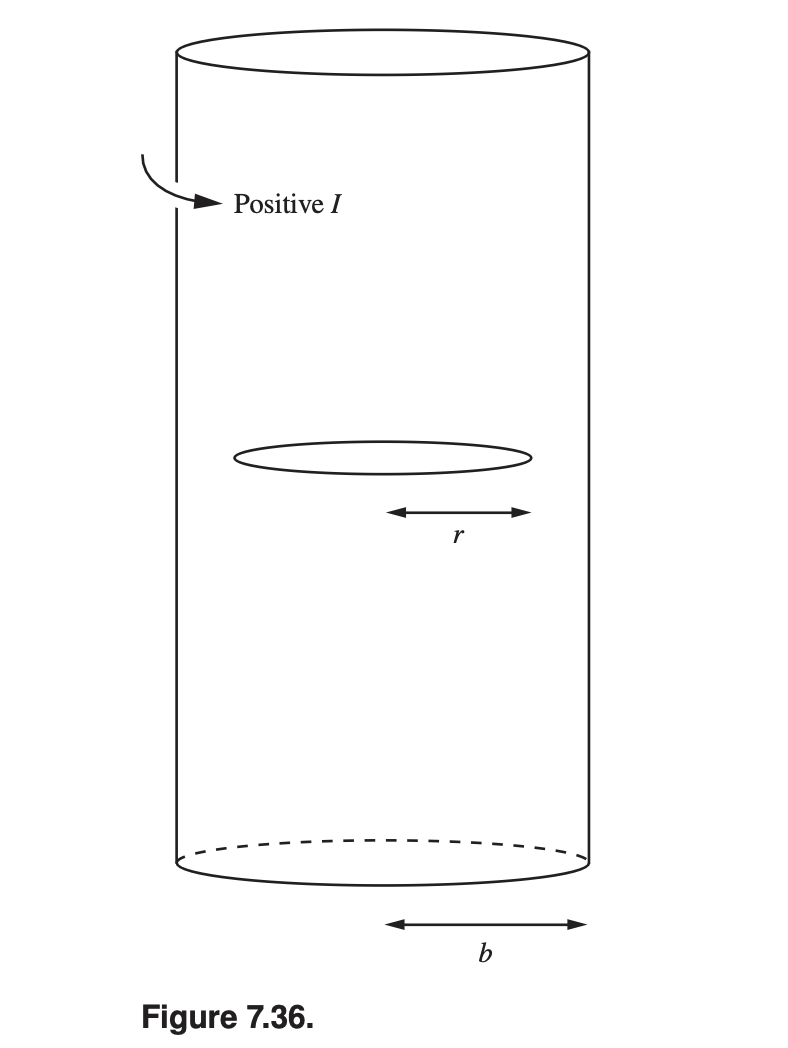
\includegraphics[width=0.4\linewidth]{F7.36.png}
\end{figure}

\vspace{5mm}
\noindent
\textbf{Solution} \, (a) The magnetic field inside the solenoid is $B(t) = \mu_0nI_0 \cos{\omega t}$. By Faraday's law the emf within the ring is
$$E = -\pi r^2\frac{\mathrm{dB}}{\mathrm{d}t} = \pi r^2 \mu_0nI_0 \omega \sin{\omega t}.$$
Therefore, the induce current is $I(t) = \pi r^2 \mu_0nI_0 \omega \sin{\omega t}/R$ and is counterclockwise when viewed from above.\\[3mm]
(b) The force applied on a little piece of the ring is 
$$F(t) = I(t)\, \mathrm{d}\vb{l} \times \vb{B} = \frac{\pi r^2 \mu_0^2 n^2 I_0^2 \omega \, \mathrm{d}l}{R} \sin{\omega t}\cos{\omega t} = \frac{\pi r^2 \mu_0^2 n^2 I_0^2 \omega \, \mathrm{d}l}{2R} \sin{2\omega t}$$
and radially outward when positive. So it is maximum outward at $\omega t = k\pi + \pi/4$, and maximum inward at $\omega t = k\pi + 3\pi/4$.\\[3mm]
(c) The force is always radial, so it will only stretch/shrink the ring.

\pagebreak

\section{Exercise 10}
\subsection{(7.36) \textit{Connecting two circuits}}
Part (a) of Fig. 7.40 shows two coils with self-inductances $L_1$ and $L_2$. In the relative position shown, their mutual inductance is $M$. The positive current direction and the positive electromotive force direction in each coil are defined by the arrows in the figure. The equations relating currents and electromotive forces are
$$\mathcal{E}_1=-L_1\frac{\mathrm{d}I_1}{\mathrm{d}t}\pm M\frac{\mathrm{d}I_2}{\mathrm{d}t} \quad \text{and} \quad \mathcal{E}_2=-L_2\frac{\mathrm{d}I_2}{\mathrm{d}t}\pm M\frac{\mathrm{d}I_1}{\mathrm{d}t}$$
(a) Given that $M$ is always to be taken as a positive constant, how must the signs be chosen in these equations? What if we had chosen, as we might have, the other direction for positive current, and for positive electromotive force, in the lower coil? \\
(b) Now connect the two coils together, as in part (b) of the figure, to form a single circuit. What is the self-inductance $L'$ of this circuit, expressed in terms of $L_1$, $L_2$, and $M$? What is the self-inductance $L''$ of the circuit formed by connecting the coils as shown in (c)? Which circuit, (b) or (c), has the greater self-inductance?\\
(c) Considering that the self-inductance of any circuit must be a
positive quantity (why couldn’t it be negative?), see if you can
draw a general conclusion, valid for any conceivable pair of
coils, concerning the relative magnitude of $L_1$, $L_2$, and $M$.
\begin{figure}[h]
    \centering
    \begin{minipage}{0.3\textwidth}
        \centering
        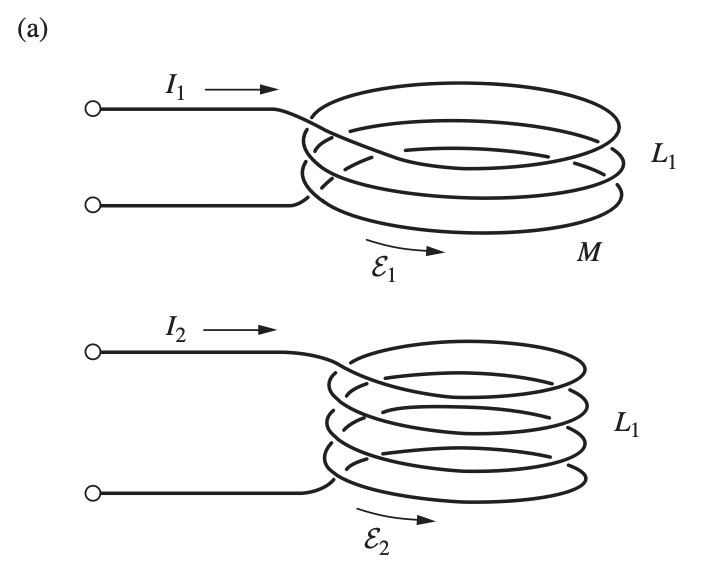
\includegraphics[width=\textwidth]{F7.40a.png}
    \end{minipage}
    \begin{minipage}{0.3\textwidth}
        \centering
        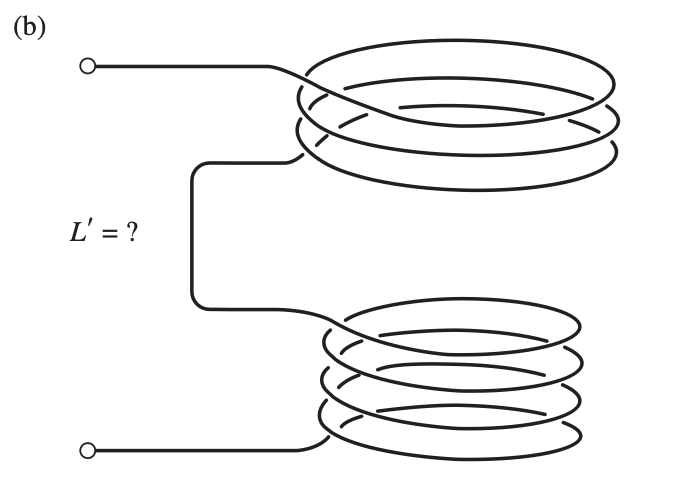
\includegraphics[width=\textwidth]{F7.40b.png}
    \end{minipage}
    \begin{minipage}{0.3\textwidth}
        \centering
        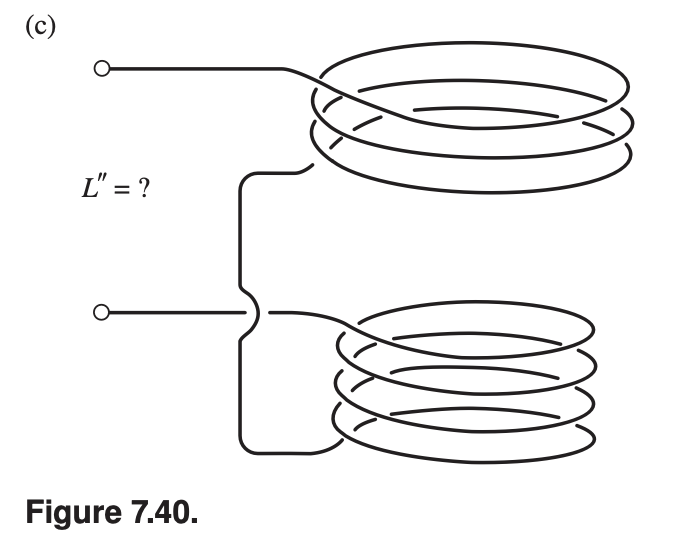
\includegraphics[width=\textwidth]{F7.40c.png}
    \end{minipage}
\end{figure}

\vspace{5mm}
\noindent
\textbf{Solution} \, (a) If $I_2$ is increasing, there will be an increasing upward flux through the upper circuit, which induces an emf in the opposite direction of $\mathcal{E}_1$. Therefore, the sign in the first equation must be $-$. Similar arguments can be made to the second equation, where the sign must also be $-$.

If we had chosen the other direction for positive current and emf in the lower coil, the sign in both equations should be $+$.\\[3mm]
(b) In part (b), $I = I_1=I_2$ and the emfs of the two circuits add, so
$$\mathcal{E} = \mathcal{E}_1+\mathcal{E}_2 =-L_1\frac{\mathrm{d}I}{\mathrm{d}t}- M\frac{\mathrm{d}I}{\mathrm{d}t} -L_2\frac{\mathrm{d}I}{\mathrm{d}t}- M\frac{\mathrm{d}I}{\mathrm{d}t} = -(L_1+L_2+2M) \frac{\mathrm{d}I}{\mathrm{d}t}.$$
Therefore, $L' = L_1+L_2+2M$.

In part (c), $I=I_1 = -I_2$  and the emfs subtracts, so
$$\mathcal{E} = \mathcal{E}_1-\mathcal{E}_2 =-L_1\frac{\mathrm{d}I}{\mathrm{d}t}- M\frac{\mathrm{d}(-I)}{\mathrm{d}t} +L_2\frac{\mathrm{d}(-I)}{\mathrm{d}t}+ M\frac{\mathrm{d}I}{\mathrm{d}t} = -(L_1+L_2-2M) \frac{\mathrm{d}I}{\mathrm{d}t}.$$
Therefore, $L'' = L_1+L_2-2M$.

Since $M$ is always positive, circuit (b) has greater self-inductance.\\[3mm]
(c) A circuit with $L < 0$ simply couldn't exist, since an increasing current within the circuit would cause an positive emf that further reinforces the current, and eventually violate the law of energy conservation. Therefore,
$$L''\geq0 \implies M\leq \frac{L_1+L_2}{2}.$$

\subsection{(8.23) \textit{Energy in an RLC circuit}}
For the damped $RLC$ circuit of Fig. 8.2, work out an expression for the total energy stored in the circuit (the energy in the capacitor plus the energy in the inductor) at any time $t$, for all three of the underdamped, overdamped, and critically damped cases; you need not simplify your answers. If $R$ is varied while $L$ and $C$ are kept fixed, show that the critical damping condition, $R= 2\sqrt{L/C}$, is the one in which the total energy is most quickly dissipated. (The exponential behavior is all that matters here.) The results from Problem 8.4 will be useful.
\begin{figure}[H]
    \centering
    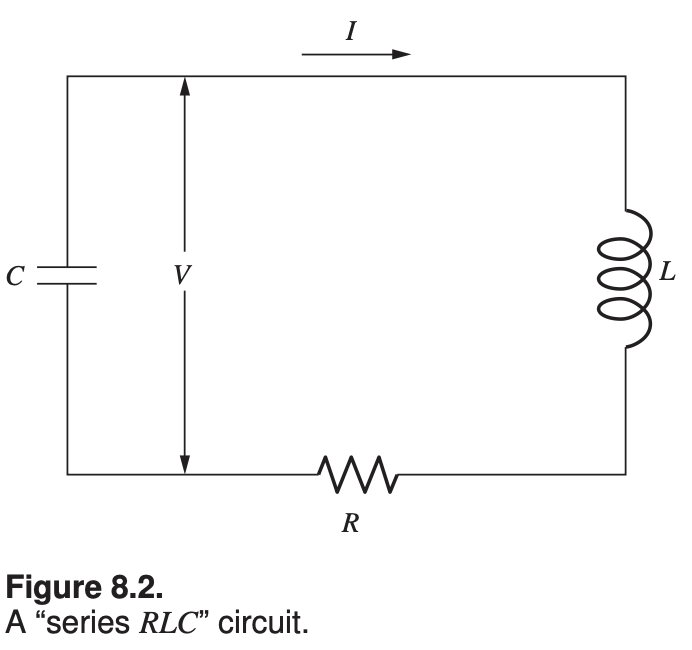
\includegraphics[width=0.4\linewidth]{F8.2.png}
\end{figure}

\vspace{5mm}
\noindent
\textbf{Solution} \, In the case of the underdamped circuit,
$$V(t) = e^{-\alpha t}(A \cos \omega t + B \sin \omega t) \implies I(t) = -C\frac{\mathrm{d}V}{\mathrm{d}t} = Ce^{-\alpha t}(A\omega \sin \omega t-B \omega \cos \omega t + A \alpha \cos \omega t + B \alpha \sin \omega t).$$
Therefore,
$$U(t) = \frac{1}{2}CV^2+\frac{1}{2}LI^2 = \frac{1}{2}Ce^{-2\alpha t}\left[\left(A \cos \omega t + B \sin \omega t\right)^2+LC\left(A\omega \sin \omega t-B \omega \cos \omega t + A \alpha \cos \omega t + B \alpha \sin \omega t\right)^2\right].$$
The energy decays like $e^{-2\alpha t}$.

In the overdamped case,
$$V(t) = Ae^{-\beta_1t} +Be^{-\beta_2t} \implies I(t) =  AC\beta_1e^{-\beta_1t} + BC\beta_2e^{-\beta_2t}.$$
Therefore,
$$U(t) = \frac{1}{2}C\left(Ae^{-\beta_1t} +Be^{-\beta_2t}\right)^2+\frac{1}{2}LC^2\left(A\beta_1e^{-\beta_1t} + B\beta_2e^{-\beta_2t}\right)^2.$$
The energy decays like $e^{-2\beta' t}$ where $\beta' = \min\left\{\beta_1, \beta_2\right\}$.

In the critically damped case,
$$V(t)=\left(A + Bt\right )e^{-\beta t} \implies I(t) = Ce^{-\beta t}\left[\beta (A + Bt)-B\right]$$
where $\beta = (LC)^{-1/2}$ as $R = 2 \sqrt{L/C}$. Therefore,
$$U(t) = \frac{1}{2}Ce^{-2\beta t}\left[(A+Bt)^2+LC\left(\beta \left(A + Bt\right)-B\right)^2\right].$$
The energy decays like $e^{-2\beta t}$.

The fact that the energy decays most quickly in the critically damped circuits can be shown by:
\begin{align*}
    \beta > \alpha & \iff \frac{1}{\sqrt{LC}} > \frac{R}{2L} \\
    & \iff R<2\sqrt{\frac{L}{C}} \\ 
    & \iff \text{underdamped}
\end{align*}
and
\begin{align*}
    \beta > \beta' & \iff \beta > \frac{R}{2L}\left(1-\sqrt{1-\frac{4L}{R^2C}}\right)\\
    & \iff \beta > \alpha - \sqrt{\alpha^2 - \beta^2} \\
    & \iff \sqrt{\alpha + \beta } > \sqrt{\alpha - \beta}
\end{align*}

\pagebreak

\section{Exercise 11} 
\subsection{\textit{Matrix method for RLC circuit}}
The 2nd order ODE for $RLC$ circuit 
$$\frac{\mathrm{d}^2Q}{\mathrm{d}t^2}+ \frac{R}{L} \frac{\mathrm{d}Q}{\mathrm{d}t}+ \frac{Q}{LC}=0$$
can also be expressed as a 1st order ODE of a vector $\vb{x}=[Q,\dot{Q}]^{\mathsf{T}}$, i.e. $\dot{\vb{x}} = A\vb{x}$. \\[3mm]
(a) Derive the dynamic matrix $A$.\\
(b) Find the eigenvalue and eigenvector of $A$.\\
(c) Discuss (b) at the critical state.

\vspace{5mm}
\noindent
\textbf{Solution} \, (a) $\dot{\vb{x}} = [\dot{Q},\ddot{Q}]^{\mathsf{T}}$, and $\ddot{Q} = -R\dot{Q}/L - Q/LC$. Therefore,
$$
\begin{bmatrix}
    \dot{Q} \\
    \ddot{Q}
\end{bmatrix}
=
\begin{bmatrix}
    0 & 1 \\
    -\frac{1}{LC} & -\frac{R}{L} 
\end{bmatrix}
\begin{bmatrix}
    Q \\
    \dot{Q}
\end{bmatrix}
\implies A = 
\begin{bmatrix}
    0 & 1 \\
    -\frac{1}{LC} & -\frac{R}{L} 
\end{bmatrix}
$$
(b) We solve the characteristic equation:
$$
\begin{vmatrix}
    \lambda I-A
\end{vmatrix}
=
\begin{vmatrix}
    \lambda & -1 \\
    \frac{1}{LC} & \lambda+\frac{R}{L}
\end{vmatrix}
= \lambda^2 + \frac{R}{L}\lambda + \frac{1}{LC} = 0
$$
Therefore, the eigenvalues are
$$\lambda_{1,2} = \frac{-R+\sqrt{R^2-\dfrac{4L}{C}}}{2L}$$

Then find the general eigenvectors for any eigenvalues $\lambda$. Let $\vb{v} = \begin{bmatrix} v_1 \\ v_2 \end{bmatrix}$,
$$
(\lambda I - A)\vb{v} = 
\begin{bmatrix}
    \lambda & -1 \\
    \frac{1}{LC} & \lambda+\frac{R}{L}
\end{bmatrix}
\begin{bmatrix} 
    v_1 \\
    v_2 
\end{bmatrix}
= 0 
\implies v_2 = \lambda v_1
$$
So the eigenvectors corresponding to the eigenvalues $\lambda_{1,2}$ are
$$
\vb{v}_{1,2} = 
\begin{bmatrix}
    1 \\
    \lambda_{1,2}
\end{bmatrix}
$$
and their scalar multiples.\\
(c) Critical damping occurs when $R^2=4L/C$, and the eigenvalues collapse into a real repeated root $\lambda = -R/2L$. Then the matrix
$$\lambda I - A = 
\begin{bmatrix}
    \lambda & -1 \\
    \frac{1}{LC} & \frac{R}{L} + \lambda
\end{bmatrix}
=
\begin{bmatrix}
    -\frac{R}{2L} & -1 \\
    \frac{1}{LC} & \frac{R}{2L}
\end{bmatrix}
$$
has rank $1$ and thus defective. It has only one eigenvector
$$\vb{v} = 
\begin{bmatrix}
    1 \\
    -\frac{R}{2L}
\end{bmatrix}
$$
Since there is only one eigenvector, the solution cannot be diagonalized. The system is solved using the Jordan form, and the general solution is:
$$\vb{x}(t) = (c_1 + c_2 t) e^{\lambda t} \vb{v}$$

\subsection{(8.21) \textit{Solving an RLC circuit}}
In the resonant circuit in Fig. 8.34 the dissipative element is a resistor $R'$ connected in parallel, rather than in series, with the $LC$ combination. Work out the equation, analogous to Eq. (8.2), that applies to this circuit. Find also the conditions on the solution analogous to those that hold in the series $RLC$ circuit. If a series $RLC$ and a parallel $R'LC$ circuit have the same $L$, $C$, and $Q$ (quality factor, not charge), how must $R'$ be related to $R$?
\begin{figure}[H]
    \centering
    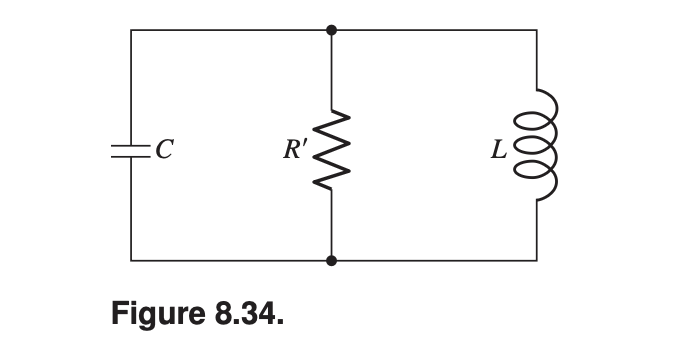
\includegraphics[width=0.5\linewidth]{F8.34.png}
\end{figure}

\vspace{5mm}
\noindent
\textbf{Solution} \, Let the voltage drop between node $B$ and $A$ be $V$, and loop currents be $I_1$ and $I_2$ as shown in the figure.
\begin{center}
\begin{circuitikz}[line width = 0.8pt]
    \draw (0,0) node[above] {$A$} to[R,l_=$R'$] (0,-3) node[below] {$B$};
    \draw (3,0) to[L,l^=$L$] (3,-3);
    \draw (-3,0) to[C,l_=$C$] (-3,-3);
    \draw (-3,0) to (0,0) to (3,0);
    \draw (-3,-3) to (0,-3) to (3,-3);

    \draw[->] (-0.8, -1.5) arc[start angle=0,end angle=350,radius=0.7];
    \node at (-1.5, -1.5) {$I_1$};
    \draw[->] (2.2, -1.5) arc[start angle=0,end angle=350,radius=0.7];
    \node at (1.5, -1.5) {$I_2$};
\end{circuitikz}
\end{center}
The following relationships hold for the circuit:
$$V=R'(I_1-I_2), \quad q=CV, \quad I_1 = -\frac{\mathrm{d}q}{\mathrm{d}t},\quad V =L\frac{\mathrm{d}I_2}{\mathrm{dt}}.$$
Therefore,
$$\frac{\mathrm{d}V}{\mathrm{d}t} = R\left(\frac{\mathrm{d}I_1}{\mathrm{d}t}-\frac{\mathrm{d}I_2}{\mathrm{d}t}\right) = R'\left(-\frac{\mathrm{d}^2q}{\mathrm{d}t^2}-\frac{V}{L}\right)=-R'C\frac{\mathrm{d}^2V}{\mathrm{d}t^2}-\frac{R'V}{L}$$
$$\implies \frac{\mathrm{d}^2V}{\mathrm{d}t^2} + \frac{1}{R'C} \frac{\mathrm{d}V}{\mathrm{d}t} + \frac{1}{CL}V = 0$$
Compare this equation to Eq. (8.2). The two would be identical by substituting $1/R'C$ for $R/L$. Hence, the conditions on the solution for the parallel $RLC$ circuits are:
$$\alpha = \frac{1}{2R'C},\quad \omega^2 = \frac{1}{LC} - \frac{1}{4R'^2C^2}.$$

If the parallel circuit above has the same $L$, $C$ and $Q=\omega/2\alpha$ as a series $RLC$ circuit, then
$$Q^2 = R'C\left(\frac{1}{LC}-\frac{1}{4R'^2C^2}\right) = \frac{L}{R} \left(\frac{1}{LC}-\frac{R^2}{4L^2}\right)\implies  R' = \frac{L}{RC}.$$

\subsection{(8.31) \textit{Zero voltage difference}}
Show that, if the condition $R_1R_2 = L/C$ is satisfied by the components of the circuit in Fig. 8.39, the difference in voltage between points A and B will be zero at any frequency. Discuss the suitability of this circuit as an ac bridge for measurement of an unknown inductance.

\begin{figure}[H]
    \centering
    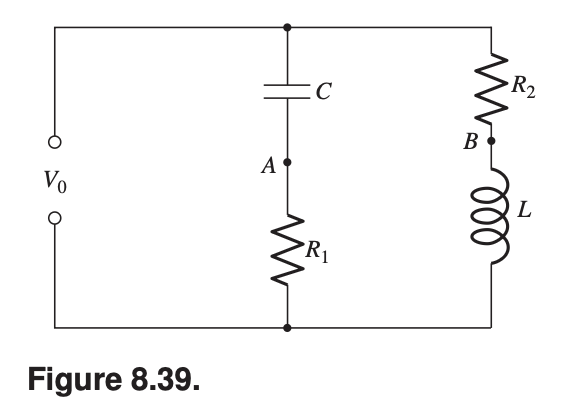
\includegraphics[width=0.4\linewidth]{F8.39.png}
\end{figure}

\vspace{5mm}
\noindent
\textbf{Solution} \, The currents through two branches are
$$I_1 =\frac{V_0}{R_1+\frac{1}{i\omega C}} \quad  \text{and} \quad I_2 = \frac{V_0}{R_2+i\omega L}.$$
Therefore, the voltages at $A$ and $B$ are

$$V_A = I_A R_1 = \frac{V_0 R_1}{R_1+\frac{1}{i\omega C}} \quad \text{and} \quad V_B = V_0-I_BR_2 = \frac{V_0i\omega L}{R_2+i\omega L}.$$
The difference vanished when
$$\frac{V_0 R_1}{R_1+\frac{1}{i\omega C}}=\frac{V_0i\omega L}{R_2+i\omega L} \implies R_1R_2 = \frac{L}{C}.$$
Given known $C$, we can adjust $R_1$ and $R_2$ until $V_B=V_A$ and deduce the unknown $L$.

\pagebreak

\section{Exercise 12}
\subsection{(9.14) \textit{Sphere with a hole}}
A current $I$ flows along a wire toward a point charge, causing the charge to increase with time. Consider a spherical surface $S$ centered at the charge, with a tiny hole where the wire is, as shown in Fig. 9.14. The circumference $C$ of this hole is the boundary of the
surface $S$. Verify that the integral form of Maxwell’s equation,
$$\int_C \vb{B} \, \mathrm{d}\vb{s} = \int_S \left(\mu_0 \varepsilon_0 \frac{\partial \vb{E}}{\partial t}+\mu_0 \vb{J}\right) \,\mathrm{d}\vb{a},$$
is satisfied.
\begin{figure}[H]
    \centering
    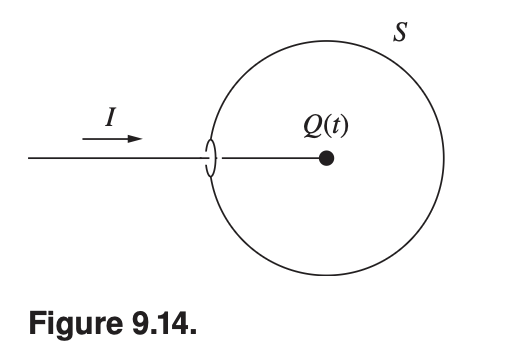
\includegraphics[width=0.35\linewidth]{F9.14.png}
\end{figure}

\vspace{5mm}
\noindent
\textbf{Solution} \, On the left side, the magnetic field in the vicinity of wire is $B = \mu_0I/2\pi r$, and thus
$$\int_C \vb{B}\,  \mathrm{d}\vb{s} = \frac{\mu_0I}{2\pi  r} \cdot 2\pi r = \mu_0I.$$
On the right side, $\vb{J}=0$ since there is no current passing through the surface $S$. The electric field on the surface is
$$E = \frac{Q}{4\pi \varepsilon_0 R^2} \implies \frac{\partial E}{\partial t} = \frac{1}{4\pi \varepsilon_0 R^2} \frac{\partial Q}{\partial t} = \frac{I}{4\pi \varepsilon_0 R^2}.$$
Therefore, 
$$\int_S \left(\mu_0\varepsilon_0 \frac{\partial \vb{E}}{\partial t}+\mu_0\vb{J}\right)\, \mathrm{d}\vb{a} = \mu_0 \varepsilon_0 \frac{I}{4\pi\varepsilon_0 R^2} \cdot 4\pi R^2= \mu_0I.$$
The integral form of Maxwell’s equation is indeed satisfied.

\subsection{(9.15) \textit{Field inside a discharging capacitor}}
The magnetic field inside the discharging capacitor shown in Fig. 9.1 can in principle be calculated by summing the contributions from all elements of conduction current, as indicated in Fig. 9.5. That might be a long job. If we can assume symmetry about this axis, it is very much easier to find the field $\vb{B}$ at a point by using the integral law,
$$\int_C \vb{B} \, \mathrm{d}\vb{s} = \int_S \left(\mu_0 \varepsilon_0 \frac{\partial \vb{E}}{\partial t}+\mu_0 \vb{J}\right) \,\mathrm{d}\vb{a},$$
applied to a circular path through the point. Use this to show that the field at $P$, which is midway between the capacitor plates in Fig. 9.15, and a distance $r$ from the axis of symmetry, equals $B=\mu_0Ir/2\pi b^2$. You may assume that the distance $s$ between the plates is small compared with their radius $b$. (Compare this with the calculation of the induced electric field $\vb{E}$ in the example of Fig. 7.16.)

\vspace{5mm}
\noindent
\textbf{Solution} \, Introducing the displacement current, the integral law can be written as
$$\int_C \vb{B} \, \mathrm{d}\vb{s} = \mu_0\int_S \left(\vb{J}_\text{d} + \vb{J}\right) \,\mathrm{d}\vb{a},$$
Inside the capacitor, $\vb{J} = 0$ and 
$$\int_S\vb{J}_\text{d}\, \mathrm{d}\vb{a}= I_P = I\frac{r^2}{b^2}.$$
\begin{figure}[H]
    \centering
    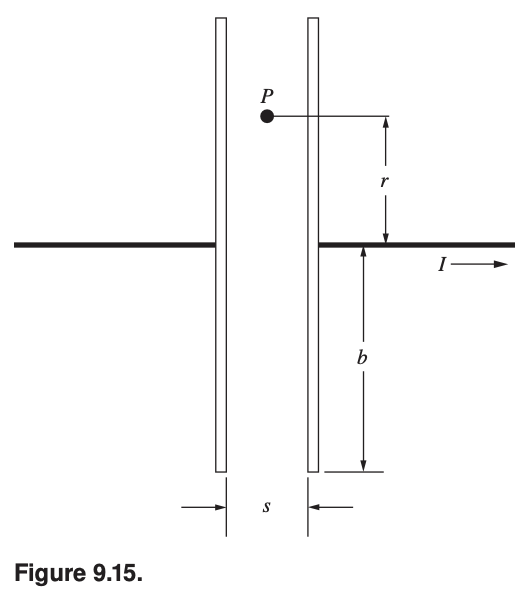
\includegraphics[width=0.4\linewidth]{F9.15.png}
\end{figure}
\noindent Therefore, 
$$2\pi r B = \mu_0I\frac{r^2}{b^2} \implies B = \frac{\mu_0Ir}{2\pi b^2}$$

\subsection{(9.22) \textit{Plane-wave pulse}}
Consider the plane-wave pulse of $\vb{E}$ and $\vb{B}$ fields shown in Fig. 9.17; $\vb{E}$ points out of the page, and $\vb{B}$ points downward. The fields are uniform inside a “slab” region and are zero outside. The slab has length $d$ in the $x$ direction and large (essentially infinite) lengths in the $y$ and $z$ directions. It moves with speed $v$ (to be determined) in the $x$ direction. This slab can be considered to be a small section of the transition shell in Appendix H. However, you need not worry about how these fields were generated. All that matters is that the electromagnetic field is self-sustaining via the two “induction” Maxwell equations\\[3mm]
(a) With the dashed rectangular loop shown (which is fixed in space, while the slab moves), use the integral form of one of Maxwell’s equations to obtain a relation between $E$ and $B$. \\
(b) Make a similar argument, with a loop perpendicular to the plane of the page, to obtain another relation between $E$ and $B$. (Be careful with the signs.) Then solve for $v$.
\begin{figure}[H]
    \centering
    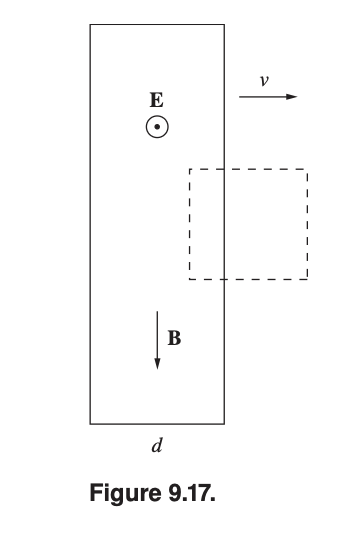
\includegraphics[width=0.3\linewidth]{F9.17.png}
\end{figure}

\vspace{5mm}
\noindent
\textbf{Solution} \, (a) Let the vertical length of the loop be $h$. Apply 
$$\oint_{\partial C} \vb{B} \, \mathrm{d}\vb{s} = \mu_0\varepsilon_0\frac{\mathrm{d}}{\mathrm{d}t}\int_C \vb{E}\,\mathrm{d}\vb{a}.$$
On the left side, only the segment inside the slab contributes, so $\oint B \, \mathrm{d}s = Bh.$ On the right side, the $E$-flux through the loop is $E\cdot(hx_\text{in})$, where $x_{\text in}$ is the instantaneous overlap of slab and loop, and it grows at rate $v$. Therefore,
$$\frac{\mathrm{d}}{\mathrm{d}t}\int_C E\,\mathrm{d}a = E h \frac{\mathrm{d} x_{\text in}}{\mathrm{d}t} = Ehv.$$
Hence, $Bh = \mu_0 \varepsilon_0 Ehv \implies B = \mu_0\varepsilon_0Ev.$\\[3mm]
(b) Now pick a rectangular loop in a plane perpendicular to the page of width $L$ in the $z$–direction and height whatever in $x$. Apply
$$\oint_{\partial C}\vb{E}\, \mathrm{d}\vb{s} =-\frac{\mathrm{d}}{\mathrm{d}t}\int_C\vb{B}\,\mathrm{d}\vb{a}.$$
On the left side, only the top edge of length $L$ sits inside the slab where $E\neq0$, so $\oint E\,\mathrm{d}s = EL$. On the right side, the $B$-flux through that loop is $B\cdot(Lx_{\text in})$, with $\mathrm{d}(x_{\text{in}})/\mathrm{d}t=v$. Therefore,
$$-\frac{\mathrm{d}}{\mathrm{d}t}\int_C B\,\mathrm{d}a = -BL\frac{\mathrm{d}x_{\text{in}}}{dt}
= -BLv.$$
Hence, $EL=-(-BLV) \implies E=Bv.$

Combine two relations between $E$ and $B$,
$$B=\mu_0\varepsilon_0 Ev, \quad E=Bv \implies v= \frac{1}{\sqrt{\mu_0\varepsilon_0}}.$$

\subsection{(9.28) \textit{Poynting vector and resistance heating}}
A longitudinal $\vb{E}$ field inside a wire causes a current via $\vb{J}=\sigma \vb{E}$. And since the curl of $\vb{E}$ is zero, this same longitudinal $\vb{E}$ component must also exist right outside the surface of the wire. Show that the Poynting vector flux through a cylinder right outside the wire accounts for the $IV$ resistance heating.

\vspace{5mm}
\noindent
\textbf{Solution} \, Let the radius of the wire be $a$. Inside the wire, Ohm’s law gives:
$$ \vb{J} = \sigma \vb{E} \implies I = J \cdot \pi a^2 = \sigma E_z \pi a^2 \implies  E_z = \frac{I}{\sigma \pi a^2}. $$
Outside the wire ($r > a$), the electric field still has a longitudinal component $E_z$ due to the continuity of the electric field from the boundary condition. The magnetic field $\vb{B}$ is purely azimuthal from Ampère’s law:
$$\vb{B} = B_\phi(r)\vu{\phi}, \quad B_\phi(r) = \frac{\mu_0 I}{2\pi r}.$$
The Poynting vector is defined as:
$$\vb{S} = \frac{1}{\mu_0} \vb{E} \times \vb{B}.$$
Substituting the fields just outside the wire:
$$\vb{S} = \frac{1}{\mu_0} (E_z \vu{z}) \times (B_\phi \vu{\phi}) = \frac{E_z B_\phi}{\mu_0} \vu{r},$$

Consider a cylindrical surface of radius $r > a$ and length $L$ coaxial with the wire. The total Poynting flux through this surface is:
\begin{align*}
    P_{\text{in}} &= \iint_{\text{surface}} \vb{S} \mathrm{d}\vb{a} = \int_0^L \int_0^{2\pi} \frac{E_z B_\phi(r)}{\mu_0} \cdot (r\, \mathrm{d}\phi\, \mathrm{d}z)\\
    &= \int_0^L \int_0^{2\pi} \frac{E_z }{\mu_0} \cdot \frac{\mu_0I}{2\pi r} \cdot (r\, \mathrm{d}\phi\, \mathrm{d}z).\\
    &= \int_0^L \int_0^{2\pi} \frac{E_z I}{2\pi} \, \mathrm{d}\phi\, \mathrm{d}z \\
    &=E_zIL 
\end{align*}
Since $E_zL =V$, we derive $P_{\text in} = IV$ as desired.

\pagebreak

\section{Exercise 13}
\subsection{(10.18) \textit{Partially filled capacitors}}
Figure 10.33 shows three capacitors of the same area and plate separation. Call the capacitance of the vacuum capacitor $C_0$. Each of the others is half-filled with a dielectric, with the same dielectric constant $\kappa$, but differently disposed, as shown. Find the capacitance of each of these two capacitors. (Neglect edge effects.)
\begin{figure}[H]
    \centering
    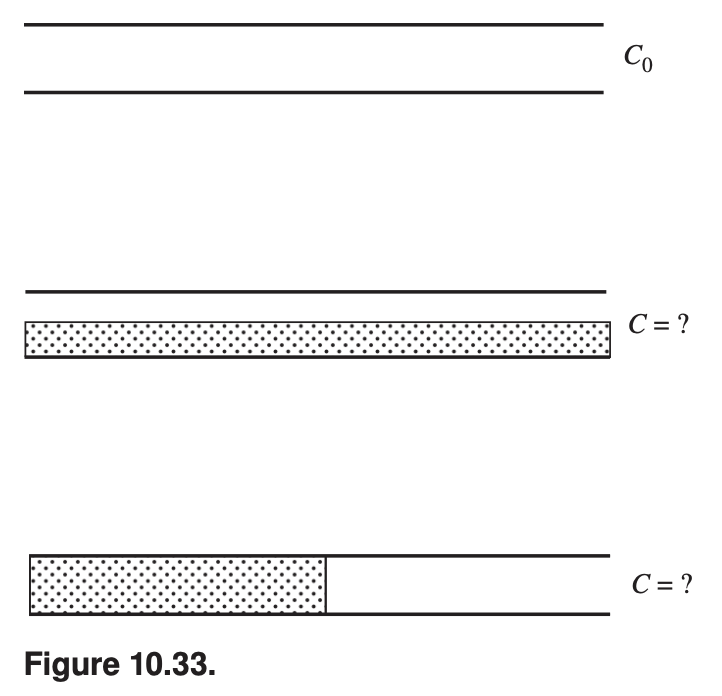
\includegraphics[width=0.4\linewidth]{F10.33.png}
\end{figure}

\vspace{5mm}
\noindent
\textbf{Solution} \, Let the area be $A$ and plate separation be $s$. Then
$$C_0=\frac{\varepsilon_0A}{s}.$$

The second capacitor is equivalent to two capacitors in series: a vacuum capacitor and a $\kappa$ dielectric capacitor both with plate separation $s/2$ and area $A$. Therefore, the total capacitance is 
$$\frac{1}{C_2} = \frac{1}{C_{21}}+\frac{1}{C_{22}} = \frac{s/2}{\varepsilon_0A}+\frac{s/2}{\kappa\varepsilon_0A} = \frac{1}{2C_0}+\frac{1}{2\kappa C_0} \implies C_2 = \frac{2\kappa}{\kappa+1}C_0.$$

The third capacitor is equivalent to two capacitors in parallel: a vacuum capacitor and a $\kappa$ dielectric capacitor both with plate separation $s$ and area $A/2$. Therefore, the total capacitance is
$$C_3 = C_{31}+C_{32} = \frac{\varepsilon_0A/2}{s}+\frac{\kappa\varepsilon_0A/2}{s} = \frac{C_0}{2} + \frac{\kappa C_0}{2} = \frac{1+\kappa}{2}C_0.$$

\subsection{(10.27) \textit{Pascal’s triangle and the multipole expansion}}
(a) If two monopoles with opposite sign are placed near each other, they make a dipole. Likewise, if two dipoles with opposite sign are placed near each other, they make a quadrupole, and so on. Explain how this fact was used in Fig. 10.36 to obtain each of the configurations from the one above it. Note that the magnitudes of the charges form Pascal’s triangle. This triangle provides a very simple way of generating successively higher
terms in the multipole expansion.\\
(b) If the bottom configuration in Fig. 10.36 is indeed an octupole, then the leading-order term in the potential at the point $P$ in Fig. 10.37 must be of order $1/r^4$. (This is two orders of $1/r$ higher than the $1/r^2$ dipole potential.) Verify this. That is, use a Taylor series to show that the order $1$, $1/r$, $1/r^2$, and $1/r^3$ terms in the potential vanish. Define $r$ to be the distance to the rightmost charge, and assume $r \gg a$. This problem is easy if you use the \texttt{Series} operation in \textit{Mathematica}, but you should work it out by hand. It is interesting to see how each of the terms vanishes. 

As you will discover, this result is related to a nice little theorem about the sum $\sum_{k=0}^N \binom{N}{k} k^m(-1)^k$, where $m$ can take on any value from $0$ to $N-1$. You are encouraged to think about this, although you don’t need to prove it here. \textit{Hint:} Expand $(1-x)^N$ with the binomial theorem, and take the derivative. Then multiply by $x$ and take the derivative again. Repeat this process as needed, and then set $x = 1$.
\begin{figure}[H]
    \centering
    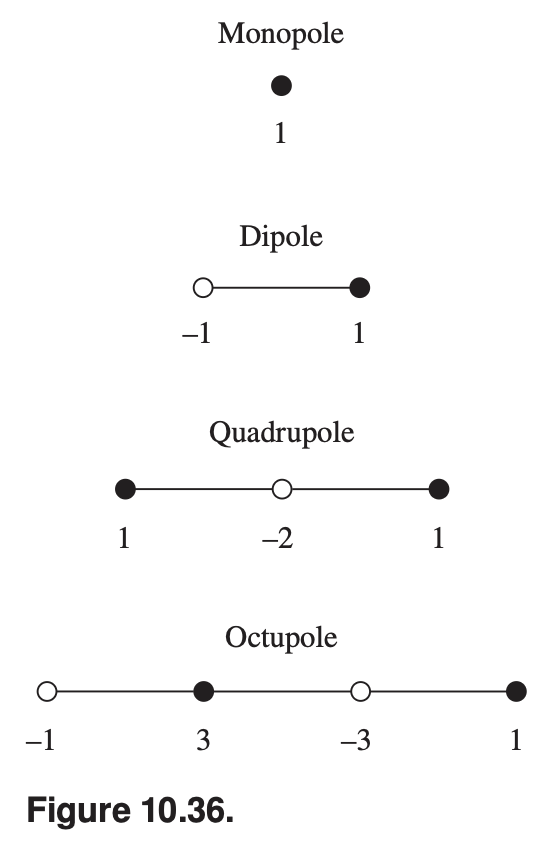
\includegraphics[width=0.3\linewidth]{F10.36.png}
\end{figure}
\begin{figure}[H]
    \centering
    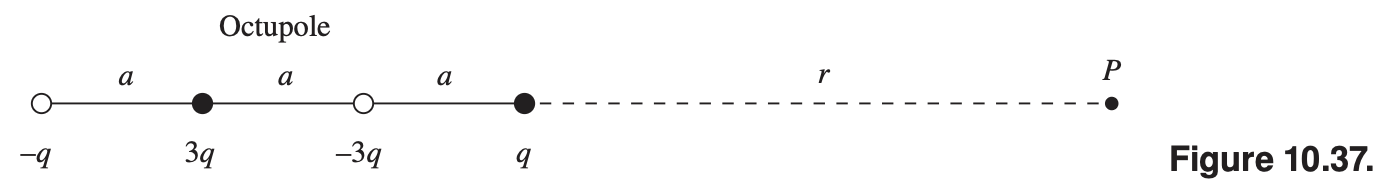
\includegraphics[width=0.8\linewidth]{F10.37.png}
\end{figure}

\vspace{5mm}
\noindent
\textbf{Solution} \, (a) Every configuration can be derived by taking a copy of the configuration above it, negating all its charges and overlapping it on the original with an offset of one unit length. \\[3mm]
(b) The potential at a point $P$ is
\begin{align*}
    \phi_P &= \frac{q}{4\pi\varepsilon_0} \left(\frac{1}{r} - \frac{3}{r+a} + \frac{3}{r+2a} - \frac{1}{r+3a} \right) \\ 
    &= \frac{q}{4\pi\varepsilon_0r} \left(1 - \frac{3}{1+a/r} + \frac{3}{1+2a/r} - \frac{1}{1+3a/r}\right)
\end{align*}
Using the Taylor series $1/(1+x) \approx 1 - x + x^2 - x^3 \quad (x\to0)$, we can expand the potential as
\begin{align*}
    \phi_P &\approx \frac{q}{4\pi\varepsilon_0r} \left[1 - 3\left(1-\frac{a}{r} + \frac{a^2}{r^2} - \frac{a^3}{r^3}\right) + 3\left(1-\frac{2a}{r} + \frac{4a^2}{r^2} - \frac{8a^3}{r^3}\right) - \left(1-\frac{3a}{r} + \frac{9a^2}{r^2} - \frac{27a^3}{r^3}\right)\right]\\
    &= \frac{q}{4\pi\varepsilon_0} \frac{6a^3}{r^4}.
\end{align*}
Indeed it is proportional to $1/r^4$.

Additionally, we can prove that the sum 
$$\sum_{k=0}^N \binom{N}{k} k^m(-1)^k$$
is nonzero only when $m=N$.  Let:
$$(1 - x)^N = \sum_{k=0}^N \binom{N}{k} (-1)^k x^k.$$
Then:
$$\sum_{k=0}^N \binom{N}{k} (-1)^k k^m = \left. \left( x \frac{d}{dx} \right)^m (1 - x)^N \right|_{x=1}.$$
This vanishes at $x = 1$ when $m < N$, but for $m = N$, it becomes:
$(-1)^N N!$

\subsection{(10.31) \textit{Mutually induced dipoles}}
Two polarizable atoms $A$ and $B$ are a fixed distance apart. The polarizability of each atom is $\alpha$. Consider the following intriguing possibility. Atom $A$ is polarized by an electric field, the source of which is the electric dipole moment $\vb{p}_B$ of atom $B$. This dipole moment is induced in atom $B$ by an electric field, the source of which is the dipole moment $\vb{p}_A$ of atom $A$. Can this happen? If so, under what conditions? If not, why not?

\vspace{5mm}
\noindent
\textbf{Solution} \, Let the distance be $r$. The field at $B$ due to $\vb{p}_A$ is $\vb{p}_A/2\pi\varepsilon_0r^3$, so the induced dipole at $B$ is $\vb{p}_B = \alpha\vb{p}_A/2\pi\varepsilon_0r^3$. In a similar manner, $\vb{p}_A = \alpha\vb{p}_B/2\pi\varepsilon_0r^3$. Therefore,
$$\vb{p}_A = \frac{\alpha^2\vb{p}_A}{4\pi^2\varepsilon_0^2r^6} \implies \vb{p}_A=0 \quad \text{or} \quad r= \left(\frac{\alpha}{2\pi\varepsilon_0}\right)^{1/3}.$$

\subsection{(10.39) \textit{Conducting-sphere limit}}
Our formula for the dielectric sphere in Section 10.10 can actually serve to describe a metal sphere in a uniform field. To demonstrate this, investigate the limiting case $\kappa \to \infty$, and show that the external field then takes on a form that satisfies the perfect-conductor boundary conditions. What about the internal field? Make a sketch of some field lines for this limiting case. What is the radius of a conducting sphere with polarizability equal to that of the hydrogen atom, given in Table 10.2?

\vspace{5mm}
\noindent
\textbf{Solution} \, The polarization of a dielectric sphere is 
$$P = \frac{3\varepsilon_0E_0(\kappa-1)}{\kappa + 2}.$$ 
In the $\kappa \to \infty$ limit, $P = 3 \varepsilon_0 E_0$. Hence, the total dipole moment of the sphere is $p = 4\pi a^3P/3 = 4\pi \varepsilon_0 a^3 E_0$. This produces a tangential field at the surface $E = p \sin \theta/4\pi \varepsilon_0a^3 = E_0 \sin \theta$, which exactly cancels the tangential component of the original field $E_0$. This satisfies the perfect-conductor boundary conditions.

The field strength inside the dielectric sphere is $E= 3E_0/(2+\kappa)$. In the $\kappa \to \infty$ limit, the field becomes zero, which is indeed correct for a conducting sphere.

Since $p=\alpha E_0$, the polarizability in this case is $\alpha = 4\pi\varepsilon_0a^3$. From the table, for the hydrogen atom $\alpha/4\pi\varepsilon_0 = a^3 = \num{0.66e-30}\si{\m \cubed}$, so a conducting sphere of equal polarizability has a radius of $(\num{0.66e-30}\si{\m \cubed})^{1/3} = \num{8.7e-11}\si{\m }$.


\end{document}